\documentclass{ieeeaccess}
\usepackage{cite}
\usepackage{amsmath,amssymb,amsfonts}
\usepackage{graphicx}
\usepackage{textcomp}
\usepackage{booktabs}
\usepackage{bm}
\usepackage{url}
% the IEEE Access class redefines \year, which pgf's random-number seed needs as a number
\let\ieeeyearsaved\year\mathchardef\year=2026
\usepackage{tikz}
\let\year\ieeeyearsaved
% loading pgf breaks the PANTONE spot color of the class (title and headings vanish): use an RGB equivalent for the class color accessblue
\definecolor{accessblue}{RGB}{0,93,148}
\usetikzlibrary{arrows.meta,calc,shadings}
\setcounter{topnumber}{4}\setcounter{totalnumber}{6}\renewcommand{\topfraction}{0.9}\renewcommand{\textfraction}{0.1}\renewcommand{\floatpagefraction}{0.7}
\newcommand{\fitcol}[1]{\footnotesize\resizebox{\ifdim\width>\columnwidth\columnwidth\else\width\fi}{!}{\input{#1}}}
\newcommand{\fitwide}[1]{\footnotesize\resizebox{\ifdim\width>\textwidth\textwidth\else\width\fi}{!}{\input{#1}}}
\makeatletter
\AtBeginDocument{\DeclareMathVersion{bold}
\SetSymbolFont{operators}{bold}{T1}{times}{b}{n}
\SetSymbolFont{NewLetters}{bold}{T1}{times}{b}{it}
\SetMathAlphabet{\mathrm}{bold}{T1}{times}{b}{n}
\SetMathAlphabet{\mathit}{bold}{T1}{times}{b}{it}
\SetMathAlphabet{\mathbf}{bold}{T1}{times}{b}{n}
\SetMathAlphabet{\mathtt}{bold}{OT1}{pcr}{b}{n}
\SetSymbolFont{symbols}{bold}{OMS}{cmsy}{b}{n}
\renewcommand\boldmath{\@nomath\boldmath\mathversion{bold}}}
\makeatother

\begin{document}
\vol{14}\year{2026}
\history{Date of publication xxxx 00, 0000, date of current version xxxx 00, 0000.}
\doi{10.1109/ACCESS.2026.XXXXXXX}

\title{Validity Threats in Data-Driven Lithium-Ion Battery State-of-Health Estimation: A Critical Review with a Controlled Evaluation-Protocol Study}
\author{\uppercase{Huy Hoang Le}\authorrefmark{1}, \uppercase{Kim-Anh Nguyen}\authorrefmark{2}}
\address[1]{[Affiliation of H. H. Le, country] (e-mail: lhhoang@powermore.vn)}
\address[2]{[Affiliation of K.-A. Nguyen, country] (e-mail: [email])}
\tfootnote{[Funding statement to be completed by the authors.]}
\markboth
{H. H. Le \headeretal: Validity Threats in Data-Driven Battery SOH Estimation}
{H. H. Le \headeretal: Validity Threats in Data-Driven Battery SOH Estimation}
\corresp{Corresponding author: Huy Hoang Le (e-mail: lhhoang@powermore.vn).}

\begin{abstract}
State of health (SOH), the share of nominal capacity that a lithium-ion cell still delivers, guides decisions on safety, replacement and reuse, and data-driven models estimate it from operating data. Studies report accuracy as an error on a test set, but this error depends on how the test set relates to the training data: it may contain further cycles of training cells, new cells, new conditions or later life. These situations pose different questions, whose effect on the reported error has rarely been measured on common data. This critical review distinguishes five evaluation questions, maps 40 recent studies onto them, and tests threats to internal, construct and external validity on four public datasets, changing one evaluation choice at a time. Withholding whole groups of cells, such as batches, instead of random cycles raised the error of boosted trees @@xjtu_LightGBM_ratio_P3_P0@@- to @@tju_LightGBM_ratio_P3_P0@@-fold on three of four datasets, because random splits place neighboring cycles of a cell in both training and test. Forecasting a cell's later life gave the highest error for boosted trees, but a factorial experiment attributes this to missing late-life data of other cells, not to temporal order. Selecting hyperparameters on the reported folds lowered the apparent error by up to @@sp_max@@ percent, and a capacity-derived input, which encodes the label, removed most of the error on two datasets but raised the held-out-batch error on a third. A reported error should therefore be read with its question, held-out unit and tuning scheme; a reporting checklist is proposed.
\end{abstract}

\begin{keywords}
battery state of health, data leakage, evaluation protocol, generalization, hyperparameter selection, lithium-ion battery
\end{keywords}

\titlepgskip=-21pt

\maketitle

\section{Introduction}
\label{sec:intro}
\PARstart{A}{ccurate} assessment of the state of health (SOH) of lithium-ion batteries is described as ``the cornerstone for ensuring the safety, reliability, and lifecycle value prediction of electric vehicles'' \cite{ma2026}. It enables users to ``optimize charging/discharging strategies, mitigate battery aging, and extend service life'' \cite{shan2025}. SOH is commonly defined as the ratio of the current capacity to a reference capacity (Section~\ref{sec:res_label}). Data-driven techniques predict this ratio from quantities measured during operation, such as features of the charging voltage curve \cite{aud12,aud17,aud31}. They ``offer superior accuracy and adaptability but often require extensive datasets'' \cite{gong2025}.

Their accuracy is reported as an error on a test set. This number, however, depends on how the test set relates to the training set. A recent review states that reported results are ``strongly affected by split design, preprocessing, and differences between training and test conditions'' \cite{sohail2026}, and published studies on the MATR dataset ``differ in at least four aspects that materially affect reported numbers'' \cite{aud53}.

The test set can relate to the training set in several ways. Its cycles can belong to cells that also supplied training cycles \cite{le2026,barua2026,maher2025}, to cells that were never seen \cite{le2026,barua2026}, or to the later life of cells whose early life was used for training \cite{aud12,aud17}. The same estimator can reach very different errors on the same data. A short conference paper reports that random splits ``yielded an R2 of up to 0.9999'' whereas group-wise cross-validation gave about 0.91 \cite{maher2025}. In our experiments, the error of LightGBM on MATR rose by a factor of @@matr_LightGBM_ratio_P3_P0@@ when whole batches were held out instead of random folds.

A reported accuracy can therefore be interpreted only together with the question that the evaluation protocol poses: ``the evaluation protocol is equally important because it determines what a reported error actually supports'' \cite{sohail2026}. The same idea has been formulated for machine learning in health, where ``the relationship between the training and the validation set should mimic the relationship between the training set and the dataset expected for the clinical use'' \cite{saeb2017}. It has also been formulated for battery lifetime prediction, where benchmarking ``should be carried out between models developed for the same use case'' \cite{geslin2023}. In this article we apply the principle to SOH estimation.

The closest existing formulation is an evaluation framework along three axes, ``Vehicles-Out, Time-Rolling, Domain-Stratified'', which a review for real-vehicle data summarizes in a short conceptual section without experiments \cite{ma2026}. We extend it to five questions and measure them on laboratory data. Our argument has three parts. First, at least five different questions are in use in the literature (Section~\ref{sec:practice}). Second, their errors are not ordered by difficulty in the way that is usually assumed. Third, conclusions about model rankings, tuning, labels and inputs do not necessarily transfer from one question to another (Section~\ref{sec:analysis}).

\subsection{Related Work and Research Gap}
The dependence of reported accuracy on the evaluation protocol is recognized, but existing work approaches it from separate directions \cite{saeb2017,sohail2026,le2026,barua2026}. General machine-learning methodology supplies the concepts. Record-wise cross-validation ``often massively overestimates'' accuracy when the use case concerns new subjects \cite{saeb2017}. A taxonomy of eight types of leakage includes temporal leakage and non-independence between training and test sets \cite{kapoor2023}, and the forecasting literature treats evaluation over time as a topic of its own \cite{hewamalage2022,bergmeir2012}. None of these works indicates how large the effects are for SOH estimation. Battery reviews and benchmarks compile what published studies report, assemble checklists \cite{sohail2026,rizanov2026} and note ``inconsistent and limited benchmarks across studies'' \cite{tan2025}. However, none of them measures how the error changes when only the protocol changes.

Controlled measurements exist for few designs, and each is limited in scope. On four NASA cells, shuffled five-fold validation has been compared with leave-one-battery-out validation \cite{le2026}. Predictor sets have been compared under random and leave-one-cell-out testing, where richer diagnostics ``can improve represented cell interpolation much more than unseen cell transfer'' \cite{barua2026}. With four cells, however, the number of independent units is too small for inference, and two mechanisms are confounded (Section~\ref{sec:res_nasa}). A short conference paper compares random splits with group-wise cross-validation \cite{maher2025}, but we had access only to its abstract. A concurrent leakage audit, not yet peer reviewed, reports that adding the charge capacity of the same cycle makes the apparent error 28 times smaller on 124 MATR cells \cite{erdogan2026}. The same audit reports that 22 of 50 highly cited papers split cycles of the same cell between training and test. Finally, a study of self-referenced features finds, under a strict online reading, ``no overall online accuracy gain'' \cite{peng2026}, which is consistent with our calibration result (Section~\ref{sec:res_calibration}). A grouped-validation framework for remaining-useful-life (RUL) and SOH prediction has also been described \cite{benabdennour2026}.

Taken together, these works compare two evaluation designs, study a single source of inflation, or describe a framework without measurements \cite{le2026,barua2026,maher2025,erdogan2026,ma2026,benabdennour2026}. How the error behaves across the full set of questions that studies pose, and with what statistical support, has remained open. We therefore do not claim as new that cell-held-out testing increases the error, that group-wise folds should be used, or that capacity-equivalent inputs inflate accuracy.

\subsection{Scope and Contributions}
This review makes four contributions (Table~\ref{tab:novelty}).
\begin{enumerate}
\item \textbf{A taxonomy of five evaluation questions.} We define five use cases of an SOH estimator (Section~\ref{sec:questions}) and map the designs of 40 recent studies onto them (Section~\ref{sec:practice}).
\item \textbf{A measurement of all five questions on common data.} We evaluate ridge regression, boosted trees and several networks on the same rows of four public datasets with 55 to 135 cells and a four-cell reference condition (Section~\ref{sec:analysis}). A factorial design separates the effect of missing late-life data of other cells from that of the target cell's own early data.
\item \textbf{Inference at the level of the independent unit.} We use exact sign-flip randomization tests, because the percentile cluster bootstrap rejected a true null too often with few groups, and we keep the bootstrap for intervals only. The analysis adds multiplicity control, a leave-one-charging-policy-out design with 70 groups, and errors that weigh every cell or group equally.
\item \textbf{The interaction of the protocol with other choices.} We examine hyperparameter selection, label reference and input features under each protocol, and we characterize held-out groups by the type of shift and by their distance from the training data.
\end{enumerate}
We identified the works above by searches of arXiv, Crossref and the web on 1 and 8 November 2026. None compares these questions on the same rows, but the search is not exhaustive, and we read the full text of only some of the works (Table~\ref{tab:novelty}).

\begin{table*}[!t]
\centering
\caption{The closest controlled studies and the present work. Entries are as stated in the full texts, repositories or abstracts available to us; the status row marks what was read.}
\label{tab:novelty}
\footnotesize
\begin{tabular}{p{0.07\textwidth}p{0.14\textwidth}p{0.16\textwidth}p{0.14\textwidth}p{0.16\textwidth}p{0.18\textwidth}}
\toprule
 & Le and Nguyen \cite{le2026} & Barua \textit{et al.} \cite{barua2026} & Maher and Yerken \cite{maher2025} & Erdo\u{g}an \cite{erdogan2026} & This work \\
\midrule
Status & journal article (authors' pilot) & journal article & 4-page conference paper (abstract only) & unreviewed manuscript and repository (repository read) & this article \\
Data & four NASA cells & four NASA cells (636 cycles); eight Oxford cells for an age-only check & ``aging data'' (not named in the abstract) & MATR (124 cells); NASA and CALCE cells; four datasets in a PINN audit (82 test cells) & NASA as reference; MATR (@@matr_cells@@ cells), HUST (@@hust_cells@@), XJTU (@@xjtu_cells@@), TJU (@@tju_cells@@) \\
Questions compared & random five-fold; leave-one-battery-out & random 80:20; leave-one-cell-out & random split; group-wise cross-validation & cell-held-out folds; proxy-feature ladder & random, cell-disjoint, held-out group, temporal, calibration, on the same rows \\
Tuning & grid of 27 combinations, five-fold CV & nested, inner leave-one-training-cell-out & not stated in the abstract & equal tuning budget per model & fixed; inner folds by cell or group; repeated inner seeds; selection on reported folds \\
Label and inputs & observed-maximum versus rated capacity & first-capacity versus rated target; predictor sets & not stated & capacity proxies as inputs & rated versus per-cell label; capacity-derived input under each protocol \\
Inference & mean and SD over folds & descriptive across cells & not stated & Wilcoxon over cells & sign-flip randomization over cells or groups; bootstrap intervals; Holm and Benjamini--Hochberg; macro-averaged errors \\
\bottomrule
\end{tabular}
\end{table*}

Two of the authors carried out a pilot study on four NASA cells \cite{le2026}. We reanalyze it as a reference condition and do not treat it as independent evidence. The remainder of the paper is organized as follows. Section~\ref{sec:questions} defines the five evaluation questions and Section~\ref{sec:practice} maps recent studies onto them. Section~\ref{sec:design} describes the design, and Section~\ref{sec:analysis} examines each threat to validity by changing one evaluation choice at a time. The remaining sections relate the findings to model families and input signals, state what the evidence supports, propose a reporting checklist, and give the limitations and conclusions.

\section{A Taxonomy of Evaluation Questions}
\label{sec:questions}
Following \cite{saeb2017}, we define a question by the relation between what the model has seen and what it is asked to estimate (Fig.~\ref{fig:overview} and Table~\ref{tab:questions}). The five questions correspond to distinct uses of an SOH estimator, and each is represented by one protocol in our experiments. Two of them resemble axes of the framework of \cite{ma2026}: a new cell (Q3) resembles ``vehicles-out'', and a forecast (Q5) resembles ``time-rolling''. Its third axis, ``domain-stratified'', performs ``training and validation within each stratum'', whereas Q4 holds a condition out. Q1 and Q2 have no counterpart in that framework, which does not mention leakage.

\begin{figure*}[!t]
\centering
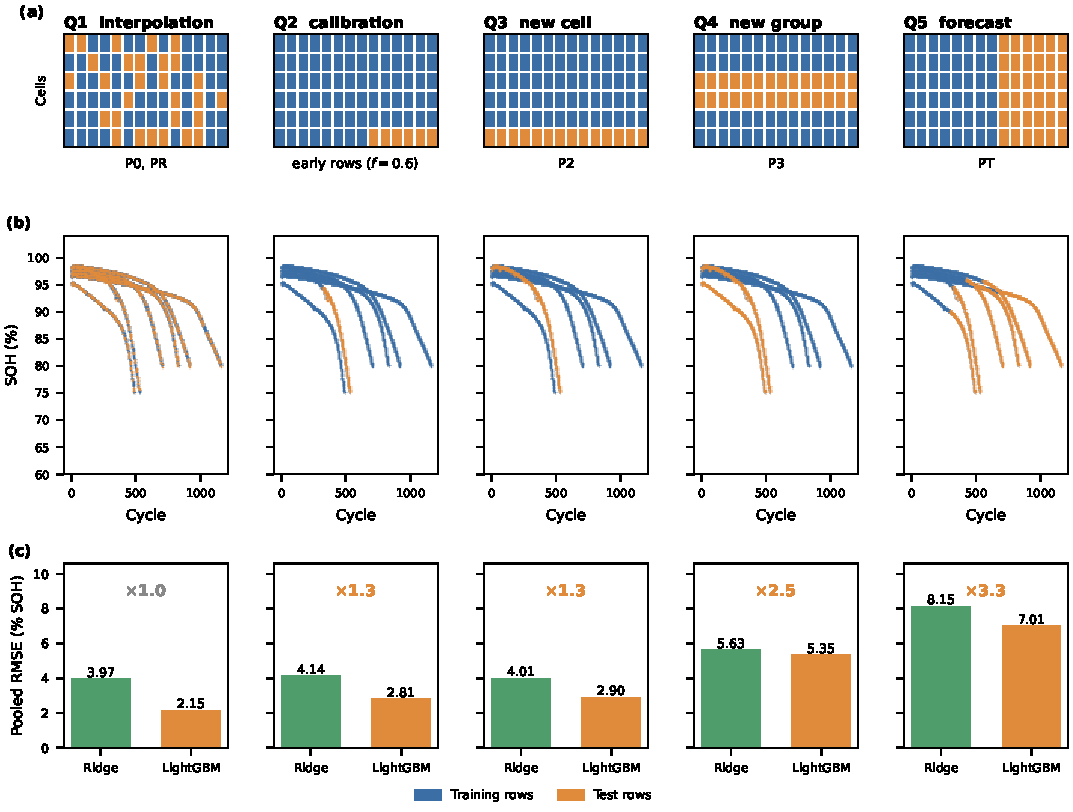
\includegraphics[width=\textwidth]{figures/fig_overview.pdf}
\caption{Overview of the five evaluation questions. (a) Schematic partitions of the cycles of six cells into training (blue) and test (orange) cycles; the protocol that represents each question in this study is named in panel B. (b) The same partitions applied to six real MATR cells (two per batch), with the SOH of every cycle plotted against the cycle number; gray lines are the full trajectories. (c) Pooled RMSE of ridge regression and LightGBM on MATR under each question (default hyperparameters, F1 features, late 40\% of each cell as test rows, early-rows column with $f=0.6$), and the ratio of the LightGBM error to its error under random folds (P0).}
\label{fig:overview}
\end{figure*}

\begin{table*}[!t]
\centering
\caption{Five evaluation questions for SOH estimation, the protocol that matches each in this study, and examples among the studies of Table~\ref{tab:practice}.}
\label{tab:questions}
\footnotesize
\begin{tabular}{p{0.04\textwidth}p{0.22\textwidth}p{0.26\textwidth}p{0.14\textwidth}p{0.20\textwidth}}
\toprule
 & Question & What the model has seen of the target & Protocol here & Studies (examples) \\
\midrule
Q1 & Estimate cycles of a cell whose other cycles, before and after, are available & cycles of the same cell on both sides of the test cycles & random folds (P0); random 60:40 within cells (PR) & \cite{aud40,aud43,aud17} \\
Q2 & Estimate later SOH of a cell when some of its own early data are labeled (calibration, fine-tuning) & the early part of the target cell & early rows added to training (calibration) & \cite{aud25,aud49} \\
Q3 & Estimate a cell never seen, drawn from the same pool as the training cells & other cells, usually including its condition & cell-disjoint folds (P2) & \cite{aud47,aud42,aud30,aud53} \\
Q4 & Estimate a cell from a condition, batch or cell type absent from training & no cell of that group & held-out group (P3) & \cite{aud31,aud45,aud01} \\
Q5 & Forecast later SOH of a cell from its earlier life & the earlier cycles of the cell (and of other cells) & temporal split (PT) & \cite{aud04,aud09,aud10,aud12,aud38,aud41} \\
\bottomrule
\end{tabular}
\end{table*}

Three assumptions about these questions are implicit in parts of the literature. First, the error increases as the model sees less of the target, from Q1 to Q4 (a \emph{difficulty ordering}) \cite{saeb2017,le2026,barua2026,maher2025}. Second, a temporal split is a safe design because it avoids ``temporal leakage'' \cite{kapoor2023}. Third, for Q2, adding early data of the target cell, as in fine-tuning \cite{aud25,aud49}, lowers the error. We examine each assumption below. The questions also differ in the independent unit, which is the cell for Q1 to Q3 and Q5 and the group of cells for Q4. Inference should follow that unit (Section~\ref{sec:design}).

We use the term leakage in a narrow sense, because four situations that are often grouped under it call for different remedies. \emph{Direct information leakage} occurs when information derived from the label or the target cell reaches the inputs or the training rows, as with a capacity-derived input (Section~\ref{sec:res_label}). \emph{Dependence} between training and test observations arises because the cycles of one cell are strongly correlated \cite{saeb2017,kaufman2012}. A \emph{mismatch of protocol} occurs when the question answered by the evaluation differs from the one that the report or application poses, for example when an error under Q1 is read as the error for a new cell. A \emph{failure to extrapolate} occurs when the test data lie outside what the training data cover (Sections~\ref{sec:res_factorial} and~\ref{sec:res_typology}). This is a property of the task and the data, not an error of the protocol. A random split by cycles is therefore not invalid in itself, since it can answer Q1. The threat arises when its result is read as evidence about new cells.

\section{Evaluation Practice in the Recent Literature}
\label{sec:practice}
\subsection{Literature Sample and Coding}
To establish which of these questions appear in current practice, we read how recent studies describe their evaluation. We started from a random-order sample of open-access preprints (arXiv) and articles (Europe PMC) from 2019 to 2026 that estimate or predict battery SOH with data-driven or hybrid methods. Records were screened on title and abstract, before any methods section was read, until 60 studies were included. For 40 of them the passage that describes the split could be read unambiguously, and these are listed in Table~\ref{tab:practice}. A script confirmed that every number and cell identifier in the table occurs in the text of the study read (three tokens differed only in spelling). A study first read as a preprint is cited by its published version when there is one. We describe the designs but do not assess the accuracy of the models.

\begin{table*}[!t]
\caption{Evaluation designs as stated in 40 of 60 recent studies. ``Held out'' is the unit left out of training as the text states it; the table does not rate any study.}
\label{tab:practice}
\centering
\footnotesize
\begin{tabular}{p{0.12\textwidth}p{0.30\textwidth}p{0.50\textwidth}}
\toprule
Study & Data & Evaluation as stated \\
\midrule
\multicolumn{3}{l}{\textit{Whole cells held out}} \\
\cite{aud47} & NASA (4 cells), Oxford (8 cells) & leave one cell out \\
\cite{aud42} & NMC cells, impedance spectra & one cell is the test set in each fold \\
\cite{aud18} & MIT, CALCE and a commercial NCA dataset & ``strict cell-level partitioning'' \\
\cite{aud30} & NASA, Stanford, HUST & splits enforced at the individual cell level \\
\cite{aud53} & MATR & 99 training cells and 24 test cells \\
\cite{aud22} & XJTU, TJU, HUST, MIT (386 batteries) & repeated battery-level protocol; five-fold cross-validation inside the training batteries \\
\cite{aud20} & CALCE, SNL & 50\% of the batteries for training, 50\% for testing \\
\cite{aud06} & five cells & all cells except the test cell for training (scenario 2) \\
\cite{aud19} & seven cells & leave one cell out; the best of five random seeds is reported \\
\cite{wang2024} & XJTU and other datasets & train on one battery, test on another; early-versus-late split of one battery is avoided to prevent leakage \\
\midrule
\multicolumn{3}{l}{\textit{One to a few cells in the test set}} \\
\cite{aud24} & NASA & B0005 and B0006 for training, B0007 for testing \\
\cite{aud32} & NASA; Oxford & B5, B6, B18 for training and B7 for testing; Oxford cells 1 to 3 for training and cell 4 for testing; the training cycles are merged and split randomly 80:20 for validation \\
\cite{aud36} & six NCA cells at different charging rates & one cell is the test set; cycles of the other five are shuffled and split 80:20 into training and validation \\
\cite{aud21} & cells 1 to 3 & cells 1 and 2 for training, cell 3 for testing \\
\cite{aud54} & CALCE, LISHEN, EVE, Oxford and others & at each charging rate, one cell for training and the other two cells for testing \\
\cite{aud25} & 19 NASA batteries & one target battery for testing; fine-tuning on 10\% of the data of the test battery \\
\cite{aud44} & CALCE CS2 (4 batteries) & leave-one-out across batteries in one experiment; the first 200 to 800 cycles as training set in another \\
\cite{aud46} & impedance spectra, four cells & cells 35C01 and 45C02 for training, 35C02 and 45C01 for testing, after removing the first 100 cycles of the test cells \\
\cite{aud52} & impedance spectra, 12 coin cells & cells split into one group for training and another for testing \\
\midrule
\multicolumn{3}{l}{\textit{Part of one cell's data used for training}} \\
\cite{aud29} & NASA group 1 (4 cells), University of Michigan data & the last 60 cycles of each cell are predicted from its preceding cycles and the data of the other three cells \\
\cite{aud38} & NASA, CALCE & first 60\% of the cycles for training and validation, remaining 40\% for testing \\
\cite{aud43} & CELL1, CELL2 & 50\% of the data of a cell for training, the rest for testing (30\% to 80\% varied); order not stated \\
\cite{aud17} & CALCE CS2 & 50\%, 60\% and 70\% of the data as training set; order not stated \\
\cite{aud04} & 12 cells & first 60\% of the life for training, last 40\% for testing; a model per cell \\
\cite{aud09} & NASA B0018 & 92 cycles for training, 40 for testing; also the first 45\% of cycles \\
\cite{aud10} & two cells & the last 8 sets of cycles left out as out-of-sample forecast \\
\cite{aud12} & NASA, four batteries & first 55\% of each battery for training, the rest for testing \\
\cite{aud41} & NASA & first 50 cycles (about 30\%) for training, the rest for validation \\
\cite{aud40} & NASA B0005; Oxford cell 2 & 144 cycles for learning and 6 for testing, the test cycles chosen at given SOH levels within the cell's life \\
\cite{aud28} & 118 cells, three datasets & four strategies: ratios within cycling conditions; ratios over the whole dataset; one temperature held out; first 80\% of each cell for training \\
\midrule
\multicolumn{3}{l}{\textit{Proportional split of pooled records}} \\
\cite{aud37} & EV battery measurements, 66,302 records & 80:20 split; whether cells are shared is not stated \\
\cite{aud60} & LiFePO$_4$ cells & 80\% of the data for training, the rest for testing; whether cells are shared is not stated \\
\cite{aud13} & NASA subsets & 70/20/10 training, validation, test; also leave-one-out across datasets \\
\cite{aud27} & synthetic and original data & 50/20/30 training, validation, test \\
\cite{aud57} & battery pack data & 50:50, 70:30 and a smaller training share \\
\midrule
\multicolumn{3}{l}{\textit{Other cell types or conditions in the test set}} \\
\cite{aud31} & 75 cells, four battery types & training on one cell at nominal conditions; testing on cells at the same or at different conditions \\
\cite{aud45} & two pouch-cell types & 3.0\,Ah cells for training, 3.5\,Ah cells for testing \\
\cite{aud49} & in-house cells and a new data set & base model trained on 8 cells; fine-tuned on one cell of the new data set \\
\cite{aud01} & three data sets & each data set can serve as test set, the other two for training \\
\cite{aud26} & NASA, 19 batteries & three training and evaluation splits (NASA-S, -M, -L) \\
\bottomrule
\end{tabular}
\end{table*}

\subsection{Findings of the Literature Reading}
Whole cells are held out in ten of the 40 studies. One of them gives the reason: training on one battery and testing on another, ``instead of training the model with early data from battery A and testing it with later data, which avoids information leakage from the training set to the test set'' \cite{wang2024}. In nine further studies the test set is one to a few cells \cite{aud24,aud32,aud21}, so that the pooled error describes only those cells (Section~\ref{sec:design}).

The studies also differ in the question that they pose. Predicting the later cycles of a cell from its earlier cycles \cite{aud38,aud43,aud17,aud28,aud29,aud44,aud04,aud09,aud10,aud12,aud41} and estimating the health of a cell never seen in training are different tasks. A study that mixes them in one paper \cite{aud28,aud44} reports numbers that should not be pooled. In transfer settings, data from the test cell enter training deliberately, for example ``with only 10\% data for fine-tuning on a testing battery'' \cite{aud25,aud49}. This is a legitimate few-shot setting, but its error answers a different question from that of a model applied to a new cell. Some studies also draw the inner validation used for tuning by shuffling cycles of the training cells \cite{aud32,aud36}. The inner scheme then does not mimic the held-out-cell deployment of the outer test.

In several studies the partition is not described in enough detail to establish what was held out. Five give a proportional split of pooled records \cite{aud37,aud60,aud13,aud57,aud27}, and for \cite{aud37} and \cite{aud60} the passages we read do not say whether cells are shared between training and test sets. Where several studies use the same dataset, their partitions differ, and a study on MATR concludes that ``cross-paper numerical comparisons should be interpreted as contextual rather than strictly apples-to-apples'' \cite{aud53}. Several studies evaluate more than one split within one paper \cite{aud28,aud26,aud57}, and some choices appear to have been made after the data had been seen. One study reports the best result of five random seeds for each case \cite{aud19}. Another chose its training cells after noting discrepancies in the spectra of one cell and removed the first 100 cycles from its test cells \cite{aud46}. A third tests on cycles picked at given SOH levels inside the life of the cell that supplies the learning cycles \cite{aud40}. Finally, the label is defined in several ways: SOH is the ratio of a capacity to the rated capacity \cite{aud25}, to the initial maximum capacity \cite{aud20} or to the initial capacity \cite{aud22} (Section~\ref{sec:res_label}).

\subsection{Implications for the Present Study}
The reading shows that studies pose different questions under the common name of validation. Whole cells are held out in a quarter of the studies, often with one to a few cells. Forecasting and the estimation of new cells are sometimes mixed, partitions are frequently not described in enough detail, and the label is defined in several ways. These observations are descriptive, and we use them as motivation. None of the designs in Table~\ref{tab:practice} is incorrect in itself, since each answers a different question. We therefore measure, on the same data and models, how much the answer changes when the question changes.

\section{Experimental Design}
\label{sec:design}
This section describes the data and the procedures common to all experiments, so that Section~\ref{sec:analysis} can be read as a sequence of single changes to one evaluation choice.


\subsection{Datasets}
Table~\ref{tab:datasets} lists the datasets. The NASA cells (B0005, B0006, B0007, B0018) \cite{saha2007} have a LiCoO\textsubscript{2} cathode \cite{le2026} and serve as the reference condition. MATR denotes the fast-charging data of Severson \textit{et al.}, who describe 124 LFP/graphite cells \cite{severson2019}. The three batch files contain @@matr_cells@@ distinct cells after we merged five cells that continue from batch~1 into batch~2 into one record. The published count of 124 is reached by also removing five cells of batch 1 and six of batch 3, as in the starter code of \cite{erdogan2026}. We kept all @@matr_cells@@ cells in the main analyses and repeated the protocol comparison on the 124 cells (Section~\ref{sec:res_protocol}). The three MATR batches contain @@matr_pol_b1@@, @@matr_pol_b2@@ and @@matr_pol_b3@@ distinct charging policies, of which @@matr_pol_12@@ are shared between batches 1 and 2 and none with batch 3. A held-out batch is therefore largely an unseen set of policies.

HUST \cite{ma2022} comprises 77 LFP/graphite cells that share one charging protocol, whereas each cell has its own four-stage discharge protocol. We formed ten groups of seven or eight cells from the cell-identifier prefix. The groups overlap in their discharge-current patterns, so a held-out HUST group is a cell-disjoint fold and not an unseen discharge protocol. XJTU \cite{wang2024} comprises 55 nickel-cobalt-manganese (NCM) cells cycled under six charging and discharging strategies. We use labels only for cycles in which capacity was measured directly. TJU \cite{zhu2022} comprises NCA, NCM and NCM+NCA 18650 cells named by cycling condition. The record we downloaded contains @@tju_cells@@ cells, whereas a study that cites it \cite{aud28} reports 118. We formed @@tju_groups@@ groups of 3 to 28 cells from the cell type and the cycling condition. The record states no rated capacity, so the \textit{Nominal} label of TJU divides by the median early capacity of the cells of the same type. We removed cycles whose capacity falls outside 55 to 105\% of the cell's own reference (under 0.2\% of the rows). No waveform features are available for TJU here, so we do not use it in the charge-curve analyses.
\begin{table}[!tb]
\centering
\caption{Datasets and held-out groups for protocol P3.}
\label{tab:datasets}
\scriptsize
\fitcol{tables/datasets.tex}
\end{table}

\subsection{Labels and Input Features}
The main label is $\mathrm{SOH}=100\,Q_\mathrm{D}/Q_\mathrm{nom}$, where $Q_\mathrm{D}$ is the measured discharge capacity of the cycle and $Q_\mathrm{nom}$ is the rated capacity (1.1\,Ah for MATR and HUST, 2.0\,Ah for XJTU). We call it the \textit{Nominal} label. The \textit{reference} label divides instead by the median capacity of the first labeled cycles of the same cell. We use three feature sets. F1 contains cycle-level quantities from the charging stage that do not contain capacity (internal resistance, temperature statistics and charge time for MATR; stage durations, charge voltages and mean constant-voltage current for HUST; analogous quantities for XJTU). F2 contains the voltage at fixed charge-capacity checkpoints of the same cycle, expressed as fractions of the rated capacity; discharge data are never used. F3 equals F1 plus the charge capacity of the cycle.

\subsection{Estimators, Protocols and Hyperparameter Selection}
We use ridge regression \cite{hoerl1970}, LightGBM \cite{ke2017}, XGBoost \cite{chen2016}, random forest \cite{breiman2001} (60 trees, 30\% subsampling) and a small multilayer perceptron (two layers of 16 units, standardized target, mean of three seeds), implemented with scikit-learn \cite{pedregosa2011} and PyTorch \cite{paszke2019}. The perceptron runs with fixed hyperparameters; a tuned variant is reported in Section~\ref{sec:res_arch}. Protocol P0 consists of five folds over pooled, shuffled cycles. In P2, five folds are formed so that all cycles of a cell fall in the same fold. P3 leaves one group of cells out (MATR batch or charging-rate bin, HUST identifier group, XJTU batch). Imputation and scaling are fitted on the training part only. We compare two regimes: fixed default hyperparameters, and hyperparameters selected by an inner three-fold cross-validation (CV) search on the training part (a small grid per model), whose inner folds hold out either cells or whole groups of cells for P3. The temporal split, the calibration design and the networks are defined where they first appear (Sections~\ref{sec:res_temporal}, \ref{sec:res_calibration} and \ref{sec:res_neural}).

\subsection{Evaluation Metric and Statistical Inference}
The primary metric is the pooled root-mean-square error (RMSE) in percentage points of SOH. In this metric a cell counts in proportion to its number of cycles. Because cells differ widely in length (170 to 2237 cycles in MATR), we also report the mean over cells of the per-cell RMSE (macro-cell RMSE) and, for held-out groups, over groups (macro-group RMSE) (Section~\ref{sec:res_macro}). They describe the error on a typical cell rather than on a typical cycle. For a pair of models, we obtain an interval for the difference in pooled RMSE by a paired percentile cluster bootstrap over independent units (cells for P0, P2 and the temporal split, held-out groups for P3). This preserves the correlation among the cycles of one cell \cite{field2007}. Grouped evaluation follows \cite{roberts2017}. P0 is a reference condition in which neighboring cycles of a cell reach the training data, a dependence between training and test observations in the sense of \cite{kaufman2012}. In addition, selecting hyperparameters on the reported folds biases the estimate, which nested validation avoids \cite{varma2006}.

We do not take P-values from the bootstrap. Resampling a small number of clusters gives intervals that are too narrow \cite{cameron2008}. In a simulation in which the two models of a pair were exchanged at random within every unit, the 95\% bootstrap interval excluded zero too often (Section~\ref{sec:res_calib}). P-values therefore come from an exact paired sign-flip randomization test \cite{ernst2004} on the per-unit totals of squared error. Under the null hypothesis that the two models are exchangeable within every unit, the sign of the per-unit difference is symmetric. We enumerate all $2^U$ sign patterns for $U\le14$ units and draw 100\,000 random patterns otherwise. The smallest two-sided $p$-value is $2^{1-U}$. At least @@gmin_1@@ units are therefore needed to reach 0.05 with a single comparison, @@gmin_6@@ with six corrected comparisons and @@gmin_91@@ with 91 (Table~\ref{tab:power}). We do not use P3 results with fewer than six groups to claim a change in ranking.

We count a sign change of the difference between two protocols as a change in ranking, and we declare it supported only if both differences have Holm-adjusted $p<0.05$ \cite{holm1979}. We report the false-discovery-rate procedure of \cite{benjamini1995} (BH) alongside. For the tabular models the family comprises all pairwise tests of one dataset and regime. For the 14 models that include networks, the primary family is the six pairs among four pre-specified main models (ridge regression, LightGBM, GRU and transformer) in each dataset and question. All 91 pairs are exploratory, and we also report one family over all datasets, questions and pairs (Section~\ref{sec:res_rank}).

\section{Critical Analysis by Threat to Validity}
\label{sec:analysis}
We group the threats by the validity question to which they belong. \emph{Internal validity} concerns whether information that the protocol is meant to exclude has reached the test set or the tuning. \emph{Construct validity} concerns whether the label and the inputs are what they appear to be. \emph{External validity} concerns whether the error carries over to other cells, conditions and settings. Table~\ref{tab:framework} maps each threat to the experiment that examines it. In each experiment we change one evaluation choice and hold data, models and features fixed.

\begin{table*}[!t]
\centering
\caption{Threats to the validity of reported SOH accuracy, where they are discussed, and where they are examined here.}
\label{tab:framework}
\footnotesize
\begin{tabular}{p{0.09\textwidth}p{0.36\textwidth}p{0.26\textwidth}p{0.2\textwidth}}
\toprule
Layer & Threat & Discussed in & Examined in \\
\midrule
Internal & Neighboring cycles of one cell on both sides of the split & \cite{rizanov2026,sohail2026} & Sec.~\ref{sec:res_nasa}, \ref{sec:res_protocol} \\
Internal & Preprocessing fitted before splitting & \cite{sohail2026} & Sec.~\ref{sec:res_selection} \\
Internal & Hyperparameters chosen on the folds that are reported & \cite{varma2006} & Sec.~\ref{sec:res_tuning}, \ref{sec:res_selection} \\
Internal & Temporal versus held-out evaluation within cells & this work & Sec.~\ref{sec:res_temporal}, \ref{sec:practice} \\
Internal & Early data of the target cell as training data & this work & Sec.~\ref{sec:res_calibration}, \ref{sec:families} \\
Internal & Ranking of models read from few independent units & this work & Sec.~\ref{sec:res_rank}, \ref{sec:res_policy} \\
Construct & Capacity reference (nominal versus measured) and label provenance & \cite{zhang2024} & Sec.~\ref{sec:res_label} \\
Construct & Inputs that encode the label (charge capacity) & this work & Sec.~\ref{sec:res_label} \\
External & Held-out cells, batches, charging policies, datasets & \cite{rizanov2026,sohail2026} & Sec.~\ref{sec:res_protocol}, \ref{sec:res_support} \\
External & Laboratory versus field duty & \cite{pozzato2023,zhao2026,ma2026} & discussion only \\
\bottomrule
\end{tabular}
\end{table*}

\subsection{Overview of the Five Evaluation Questions}
\label{sec:overview}
Figure~\ref{fig:resultmap} puts the five questions side by side. For each of the four larger datasets, it shows the pooled RMSE of ridge regression, LightGBM, a GRU and a transformer (default hyperparameters, F1 features, rated label; the networks are described in Section~\ref{sec:res_neural}). The protocols are random 60:40 splits within cells (Q1), random five-fold (P0, Q1), early rows of the target cell added to training (Q2, $f=0.6$), cell-disjoint folds (P2, Q3), held-out groups (P3, Q4) and the temporal split (Q5). All but the random split are scored on the same late rows of each cell.

\begin{figure*}[!t]
\centering
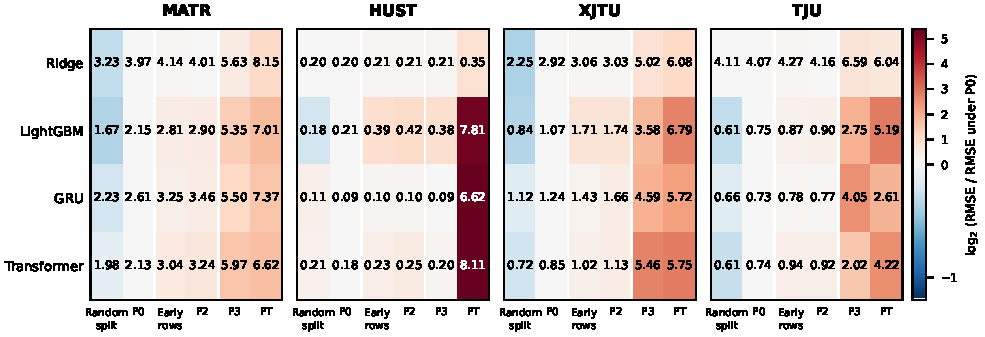
\includegraphics[width=\textwidth]{figures/fig_resultmap.pdf}
\caption{Map of the pooled RMSE (\% SOH) of ridge regression, LightGBM, a GRU and a transformer under the five questions on the four larger datasets. Cell values are the RMSE; the color is the base-2 logarithm of the ratio to the error of the same model under random folds (P0). Random split: random 60:40 split within cells; early rows: $f=0.6$ added by concatenation. All columns except the first are scored on the same late 40\% of each cell.}
\label{fig:resultmap}
\end{figure*}

The difficulty ordering holds for the boosted model with one exception. For LightGBM the error increases from the random split to random folds, to a new cell and to a new group on MATR (@@tmp_matr_LightGBM_PR@@, @@tmp_matr_LightGBM_P0@@, @@tmp_matr_LightGBM_P2@@, @@tmp_matr_LightGBM_P3@@), XJTU and TJU. The exception is HUST. There a held-out identifier group (@@tmp_hust_LightGBM_P3@@) is not more difficult than a held-out cell (@@tmp_hust_LightGBM_P2@@), which is consistent with the fact that the HUST groups are not distinct conditions.

The gap between questions appears to reflect how much of a cell a model can memorize. Ridge regression changes much less than LightGBM between the random split and a new cell (on TJU from @@tmp_tju_Ridge_PR@@ to @@tmp_tju_Ridge_P2@@, against @@tmp_tju_LightGBM_PR@@ to @@tmp_tju_LightGBM_P2@@). A small gap is therefore not evidence of a safe design. It can also reflect a model that does not use cell-specific information and whose error may be high under every question.

\subsection{Internal Validity}
\label{sec:internal}
The experiments begin with a reference condition on four NASA cells and with the effect of the protocol and of the weighting of cells (Sections~\ref{sec:res_nasa} to~\ref{sec:res_macro}). They continue with forecasting and early data of the target cell (Sections~\ref{sec:res_temporal} to~\ref{sec:res_arch}) and end with ranking stability and hyperparameter selection (Sections~\ref{sec:res_rank} to~\ref{sec:res_selection}).

\subsubsection{Reference Condition on Four NASA Cells}
\label{sec:res_nasa}
We reproduced the comparison of random five-fold validation and leave-one-battery-out (LOBO) validation of \cite{le2026} (Table~\ref{tab:nasa}). LightGBM and CatBoost \cite{prokhorenkova2018} were reproduced exactly, random forest differed slightly and XGBoost by more, for reasons that we did not isolate. The mean increase of the error under LOBO is @@nasa_mean_increase@@\% against the published @@nasa_pub_mean@@\%. With only four cells, however, two mechanisms are confounded. We cut each cell into blocks of $b$ consecutive cycles and assigned whole blocks to folds. The error grows steadily with $b$ although every cell remains in the training set (Fig.~\ref{fig:block}). For XGBoost the RMSE rises from @@block_xgb_b1@@ at $b=1$ to @@block_xgb_b64@@ at $b=64$, against @@block_xgb_lobo@@ for LOBO (LightGBM: @@block_lgb_b1@@, @@block_lgb_b64@@, @@block_lgb_lobo@@). Long blocks also remove part of the SOH range from training. The two effects therefore cannot be separated here, and a substantial part of the gap between shuffled folds and LOBO can arise without any unseen cell.
\begin{table}[!tb]
\centering
\caption{NASA cells: published and reproduced RMSE (\% SOH) for random five-fold (5-fold) and leave-one-battery-out (LOBO).}
\label{tab:nasa}
\scriptsize
\fitcol{tables/nasa.tex}
\end{table}
\begin{figure}[t]
\centering
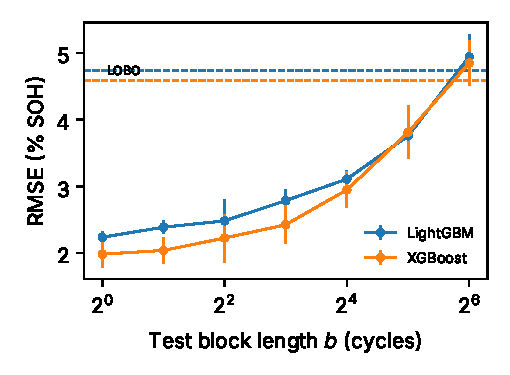
\includegraphics[width=\columnwidth]{figures/nasa_block.pdf}
\caption{NASA cells: RMSE versus length of the test blocks (mean and standard deviation over ten random block assignments). Dashed lines: leave-one-battery-out.}
\label{fig:block}
\end{figure}

\subsubsection{Effect of the Evaluation Protocol and Weighting of Cells}
\label{sec:res_protocol}
\label{sec:res_macro}
Table~\ref{tab:protocol} and Fig.~\ref{fig:protocols} give the pooled RMSE with fixed hyperparameters and F1 features. For LightGBM, the ratio of the P3 error to the P0 error was @@matr_LightGBM_ratio_P3_P0@@ on MATR, @@xjtu_LightGBM_ratio_P3_P0@@ on XJTU, @@hust_LightGBM_ratio_P3_P0@@ on HUST (absolute values below one percentage point) and @@tju_LightGBM_ratio_P3_P0@@ on TJU. Ridge regression changed much less on MATR, HUST and TJU (ratios @@matr_Ridge_ratio_P3_P0@@, @@hust_Ridge_ratio_P3_P0@@ and @@tju_Ridge_ratio_P3_P0@@; on TJU its error is already high under P0, @@tju_Ridge_P0@@), but not on XJTU (@@xjtu_Ridge_ratio_P3_P0@@).

The effect also depends on how the groups are formed. Holding out charge-rate bins instead of batches lowered the P3 error of LightGBM on MATR from @@matr_LightGBM_P3@@ to @@crate_lgb_default@@. In contrast, it raised the error on XJTU (1C, 2C, 3C; from @@xjtu_LightGBM_P3@@ to @@cr_xjtu_LightGBM@@) and on TJU (0.25C, 0.5C, 1C; from @@tju_LightGBM_P3@@ to @@cr_tju_LightGBM@@). HUST has a single charging protocol. On the 124 cells of the published description, the LightGBM errors under P0, P2 and P3 were @@m124_LightGBM_P0@@, @@m124_LightGBM_P2@@ and @@m124_LightGBM_P3@@. None of the errors of LightGBM or ridge regression differed from the values for 135 cells by more than 0.2 points.
\begin{table}[!tb]
\centering
\caption{Pooled RMSE (\% SOH), fixed hyperparameters, F1 features. P3 uses MATR batches, HUST identifier groups, XJTU batches and TJU type-by-condition groups; the last column holds out charge-rate bins (MATR: five bins; XJTU: 1C, 2C and 3C; TJU: 0.25C, 0.5C and 1C). n/a: HUST has a single charging protocol.}
\label{tab:protocol}
\scriptsize
\fitcol{tables/protocol_rmse.tex}
\end{table}
\begin{figure*}[t]
\centering
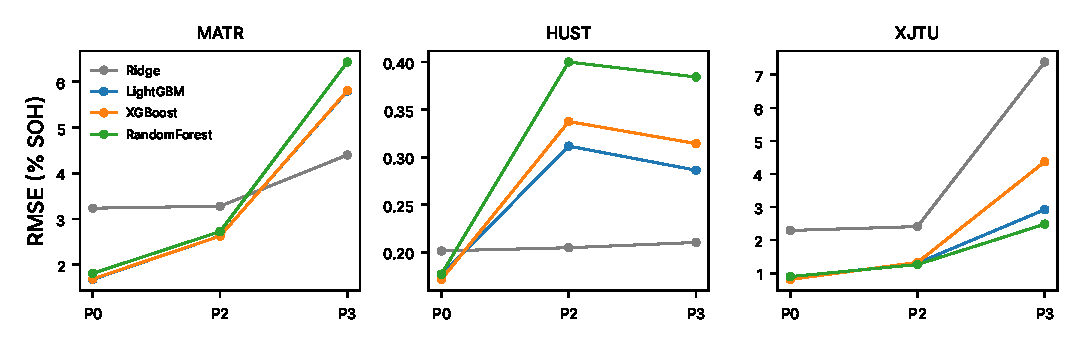
\includegraphics[width=0.85\textwidth]{figures/protocols.pdf}
\caption{Pooled RMSE by protocol for each dataset (fixed hyperparameters, F1 features).}
\label{fig:protocols}
\end{figure*}

Pooled RMSE weights every cycle equally, so that on MATR a cell of 2237 cycles counts thirteen times as much as one of 170. We therefore repeated the comparison of the four questions with the macro-cell RMSE (and, for P3, the macro-group RMSE) on the last 40\% of each cell (Table~\ref{tab:macro}). The direction of the main findings did not depend on the weighting. For LightGBM the macro-cell error of the temporal forecast exceeded that of held-out groups on all four datasets, with intervals that excluded zero (by @@mac_matr_LightGBM_ptp3@@ points on MATR, @@mac_hust_LightGBM_ptp3@@ on HUST, @@mac_xjtu_LightGBM_ptp3@@ on XJTU and @@mac_tju_LightGBM_ptp3@@ on TJU).

However, the size of the protocol effect did change. The ratio of the P3 to the P0 macro-cell error over all rows was @@mac_matr_LightGBM_ratio@@ on MATR, @@mac_hust_LightGBM_ratio@@ on HUST, @@mac_xjtu_LightGBM_ratio@@ on XJTU and @@mac_tju_LightGBM_ratio@@ on TJU (95\% interval on TJU @@mac_tju_LightGBM_ratio_lo@@ to @@mac_tju_LightGBM_ratio_hi@@), against the pooled ratios above. The order of the models changed for @@mac_flips@@ of @@mac_pairs@@ model pairs (@@mac_pct@@\%). The rank correlation between the two orders was @@mac_rho_min@@ for @@mac_rho_min_where@@, where a few long-lived cells dominate the pooled error. A report should state whether its error is pooled over cycles or averaged over cells.
\begin{table*}[!t]
\centering
\caption{Pooled and macro-cell RMSE (\% SOH) on the last 40\% of each cell for LightGBM, ridge regression and the GRU. Spearman: rank correlation between the orders of the models under the two metrics; pairs flipped: model pairs whose order differs (of 28 pairs for P0 and 91 for the other questions).}
\label{tab:macro}
\scriptsize
\fitwide{tables/macro.tex}
\end{table*}

\subsubsection{Forecasting, Training-Pool Coverage and Early Data of the Target Cell}
\label{sec:res_temporal}
\label{sec:res_factorial}
Many studies in Table~\ref{tab:practice} train on the first part of each cell's life and test on the rest. This poses a forecasting question, because the model must produce SOH values lower than those seen in training. In the temporal protocol (PT), the first 60\% of the cycles of every cell, pooled over cells, train the model and the last 40\% are the test rows. The random protocol (PR) assigns the cycles of each cell to the same proportions at random (three seeds). We scored P0, P2 and P3 on the same last 40\% of each cell (default hyperparameters, F1 features, rated label).
\begin{table}[!tb]
\caption{Pooled RMSE (\% SOH): random and temporal 60:40 splits within cells, and P0, P2 and P3 scored on the last 40\% of each cell (the temporal test rows). Default hyperparameters, F1 features, rated label.}
\label{tab:temporal}
\centering
\fitcol{tables/temporal.tex}
\end{table}

Forecasting produced the largest error of all protocols for tree ensembles on every dataset (Table~\ref{tab:temporal}). For LightGBM, the error rose from @@tmp_matr_LightGBM_PR@@ under random 60:40 to @@tmp_matr_LightGBM_PT@@ under the temporal split on MATR, from @@tmp_hust_LightGBM_PR@@ to @@tmp_hust_LightGBM_PT@@ on HUST, from @@tmp_xjtu_LightGBM_PR@@ to @@tmp_xjtu_LightGBM_PT@@ on XJTU and from @@tmp_tju_LightGBM_PR@@ to @@tmp_tju_LightGBM_PT@@ on TJU. For comparison, the errors under held-out groups were @@tmp_matr_LightGBM_P3@@, @@tmp_hust_LightGBM_P3@@, @@tmp_xjtu_LightGBM_P3@@ and @@tmp_tju_LightGBM_P3@@ on the same datasets. The ordering held for every training share between 40 and 80\% (Table~\ref{tab:tprop}; LightGBM, @@tp_gt@@ of @@tp_n@@ combinations).

The first explanation we examined is extrapolation (Fig.~\ref{fig:extrap}). Many test values lie below the range of the training values, where random forests are known to perform poorly \cite{zhang2019rerf}. The share of test rows below the lowest training SOH was @@tmprng_matr_below@@\% on MATR, @@tmprng_hust_below@@\% on HUST, @@tmprng_xjtu_below@@\% on XJTU and @@tmprng_tju_below@@\% on TJU. The LightGBM RMSE on these rows was @@rs_hust_LightGBM_out@@ on HUST, @@rs_xjtu_LightGBM_out@@ on XJTU and @@rs_matr_LightGBM_out@@ on MATR, against @@rs_hust_LightGBM_in@@, @@rs_xjtu_LightGBM_in@@ and @@rs_matr_LightGBM_in@@ on the in-range rows (Table~\ref{tab:range}). In contrast, models that extrapolate smoothly had a low out-of-range error on HUST (ridge regression @@rs_hust_Ridge_out@@, TCN @@rs_hust_TCN_out@@). A hybrid in which LightGBM models the residuals of a ridge regression lowered the temporal error on HUST from @@tmp_hust_LightGBM_PT@@ to @@iv_hust_Ridge_plus_LightGBM_PT@@ and on XJTU from @@tmp_xjtu_LightGBM_PT@@ to @@iv_xjtu_Ridge_plus_LightGBM_PT@@. It left the error unchanged on MATR and raised it on TJU.

TJU does not fit this explanation, since none of its test rows lies below the training range. However, its late rows differ from the training rows in the charge-stage features (by @@fs_tju_v_cc_start@@ standard deviations in the voltage at the start of the constant-current phase). Adding the cycle number lowered the temporal error of LightGBM on TJU from @@cyc_tju_LightGBM_PT_F1@@ to @@cyc_tju_LightGBM_PT_plus@@. Self-referenced inputs (each F1 feature minus its median over the first ten cycles of the cell) lowered it on MATR from @@sr_matr_LightGBM_PT_F1@@ to @@sr_matr_LightGBM_PT_plus@@, on XJTU from @@sr_xjtu_LightGBM_PT_F1@@ to @@sr_xjtu_LightGBM_PT_plus@@ and on TJU from @@sr_tju_LightGBM_PT_F1@@ to @@sr_tju_LightGBM_PT_plus@@. Extrapolation therefore explains the temporal result on HUST, largely on XJTU and only in part on MATR. A drift of the charge features contributes on TJU, and the remaining TJU error is not explained.
\begin{figure*}[!t]
\centering
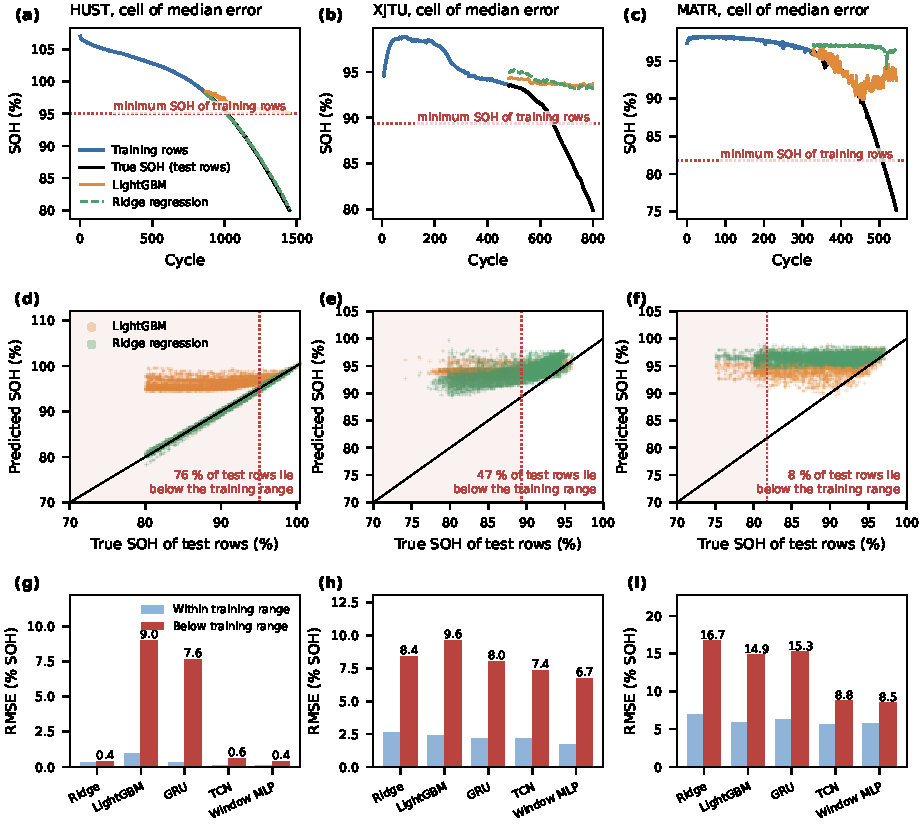
\includegraphics[width=\textwidth]{figures/fig_extrap.pdf}
\caption{Mechanism of the temporal result. (a)--(c) One cell of median error in each dataset: training rows (blue), true SOH of the test rows (black), and the predictions of LightGBM (orange) and ridge regression (dashed green); the dotted line is the lowest SOH among the training rows of all cells. (d)--(f) Predicted against true SOH for a random sample of 5000 test rows; the shaded region lies below the training range. (g)--(i) RMSE on test rows within and below the training range for five models (LGBM: LightGBM; w-MLP: window MLP). Predictions of LightGBM stop declining near the lowest training SOH.}
\label{fig:extrap}
\end{figure*}
\begin{table}[!tb]
\caption{RMSE (\% SOH) of the temporal forecast on late rows whose SOH lies within or below the range of the training rows. The column ``Share below'' gives the share of late rows with an SOH below the training range; n/a: no late row of TJU lies below the training range.}
\label{tab:range}
\centering
\fitcol{tables/range_split.tex}
\end{table}
\begin{table}[!tb]
\caption{Pooled RMSE (\% SOH) of the temporal split (PT) and of P3 and P2 scored on the same rows, for training shares of 40 to 80\% of the life of every cell. Default hyperparameters, F1 features, rated label.}
\label{tab:tprop}
\centering
\scriptsize
\fitcol{tables/tprop.tex}
\end{table}


The comparison of a temporal split with a new-cell design changes two things at once. Under P2 the other cells contribute their whole life, including the low-SOH rows of late life, and the target cell contributes nothing. Under the temporal split every cell, the target included, contributes only its first 60\%. We therefore varied independently the share $c$ of the life of the non-target cells and the share $f$ of the target cell available for training (Fig.~\ref{fig:factorial}; cell-disjoint partitions of the calibration design below, four tabular models, default hyperparameters). The corners are A ($c=1$, $f=0$), a new cell with full-life pool (P2); B ($c=0.6$, $f=0$), a new cell without late-life data in the pool; C ($c=1$, $f=0.6$), early rows of the target added to a full-life pool; and D ($c=0.6$, $f=0.6$), the temporal forecast.
\begin{figure*}[!t]
\centering
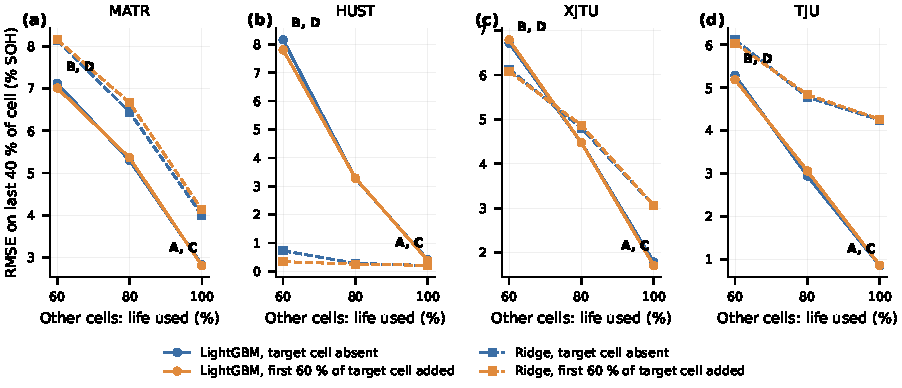
\includegraphics[width=\textwidth]{figures/fig_factorial.pdf}
\caption{Factorial separation of the coverage of late life and the early data of the target cell. Pooled RMSE on the last 40\% of each fold cell against the share of the life of the other cells that is available for training, without (blue) and with (orange) the first 60\% of the target cell; LightGBM (solid) and ridge regression (dashed). Corners A to D are defined in the text; the points at 60\% without and with the target rows are B and D, and those at 100\% are A and C.}
\label{fig:factorial}
\end{figure*}

Removing the late life of the other cells raised the LightGBM error (B minus A) by @@fx_matr_LightGBM_coverage_alone@@ points on MATR, @@fx_hust_LightGBM_coverage_alone@@ on HUST, @@fx_xjtu_LightGBM_coverage_alone@@ on XJTU and @@fx_tju_LightGBM_coverage_alone@@ on TJU (Table~\ref{tab:factorial}). In contrast, adding the first 60\% of the target cell to a full-life pool (C minus A) changed it by @@fx_matr_LightGBM_target_alone@@, @@fx_hust_LightGBM_target_alone@@, @@fx_xjtu_LightGBM_target_alone@@ and @@fx_tju_LightGBM_target_alone@@ points, at most @@fx_target_abs_max@@ in absolute value for any of the three tree ensembles. We averaged over the two orders in which the factors can be added. The share of the gap D minus A attributable to coverage was then between @@fx_share_min@@ and @@fx_share_max@@ for LightGBM, XGBoost and random forest on every dataset and for ridge regression on MATR, XJTU and TJU. The one setting in which the target rows mattered was ridge regression on HUST, where the total gap was only @@fx_hust_Ridge_total@@ points.

A new cell scored with a truncated pool (B) had practically the same error as the forecast (D), within 0.4 points. The error rose steadily as more late life was withheld (LightGBM on MATR with $f=0$: @@fx_matr_LightGBM_c10@@, @@fx_matr_LightGBM_c8@@ and @@fx_matr_LightGBM_c6@@ for $c=1$, 0.8 and 0.6). Only @@fx_matr_unc_B@@\% (MATR) and @@fx_tju_unc_B@@\% (TJU) of the test rows of B lie below the lowest training SOH, so on these datasets the missing coverage also affects rows within the training range. We conclude that the greater difficulty of forecasting than of estimating a new cell is accounted for by the absence of late-life data from the training pool. It is not explained by the temporal order of the split or by the missing history of the target cell. A temporal split is informative as a test of extrapolation, not of dependence over time.
\begin{table*}[!t]
\centering
\caption{Pooled RMSE (\% SOH) on the last 40\% of each fold cell for the corners of the factorial design (A: other cells whole life, target absent; B: other cells first 60\%, target absent; C: other cells whole life, first 60\% of target; D: all cells first 60\%), the difference D minus A with its 95\% cluster-bootstrap interval over cells, and the share of this difference attributable to coverage (average of the two orders of adding the factors; not defined when the interval of the difference includes values below 1 point).}
\label{tab:factorial}
\scriptsize
\fitwide{tables/factorial.tex}
\end{table*}

\label{sec:res_calibration}
Fine-tuning and calibration studies allow the model to see part of the target cell before it is tested \cite{aud25,aud49}. In our calibration design (cell-disjoint five-fold partitions, two random partitions), the training set comprises all rows of the cells outside the fold plus the first fraction $f$ of the rows of every cell inside the fold. The test rows are the last 40\% of each fold cell, and $f=0$ corresponds to P2 scored on the same rows. A ridge model fitted to the early rows of the target cell alone serves as comparison (Table~\ref{tab:calibration}).

The early rows changed the error of pooled models very little. For LightGBM, going from $f=0$ to $f=0.6$ changed the RMSE from @@cal_matr_LightGBM_0p0@@ to @@cal_matr_LightGBM_0p6@@ on MATR, from @@cal_hust_LightGBM_0p0@@ to @@cal_hust_LightGBM_0p6@@ on HUST, from @@cal_xjtu_LightGBM_0p0@@ to @@cal_xjtu_LightGBM_0p6@@ on XJTU and from @@cal_tju_LightGBM_0p0@@ to @@cal_tju_LightGBM_0p6@@ on TJU. Only on XJTU did the interval of the difference exclude zero. Weighting the target rows tenfold did not improve LightGBM, and the per-cell ridge model was less accurate than pooled LightGBM at every $f$. The early record was useful, however, as a reference for the cell's own inputs. Self-referenced inputs lowered the LightGBM error under P2 on MATR from @@sr_matr_LightGBM_P2_F1@@ to @@sr_matr_LightGBM_P2_plus@@ and on XJTU from @@sr_xjtu_LightGBM_P2_F1@@ to @@sr_xjtu_LightGBM_P2_plus@@, consistent with the finding of \cite{peng2026} that references matter. A claim that fine-tuning helps should therefore be accompanied by a baseline that receives the same target rows and a training pool that contains late-life data.
\begin{table}[!tb]
\caption{RMSE (\% SOH) on the last 40\% of the rows of the fold cells when the first fraction $f$ of the rows of each target cell is added to training. Default hyperparameters, F1 features, rated label. Target-only ridge uses the early rows of the cell alone.}
\label{tab:calibration}
\centering
\fitcol{tables/calibration.tex}
\end{table}

\subsubsection{Networks: Cycle History, Fine-Tuning Schedules and Architectures}
\label{sec:res_neural}
\label{sec:res_schedules}
\label{sec:res_arch}
Many studies in Table~\ref{tab:practice} use sequence models that read several preceding cycles \cite{aud24,aud26,aud01,aud13}. We trained a gated recurrent unit (GRU) network \cite{cho2014} (one layer of 32 units) and a small transformer encoder \cite{vaswani2017} (two layers of width 32, four attention heads) without tuning. Both read windows of the 10 most recent cycles of the F1 features of a cell (Adam \cite{kingma2015}, learning rate $2\times10^{-3}$, 12 epochs, batch 512, every first, second or fourth training row depending on data size). We evaluated them under all five questions (Table~\ref{tab:neural}). In the early-rows design they were trained on the concatenated data or fine-tuned for three epochs on the early rows of the fold cells (learning rate $3\times10^{-4}$, all weights).
\begin{table}[!tb]
\caption{RMSE (\% SOH) of ridge regression, LightGBM, a GRU and a transformer under the five questions, scored on the last 40\% of each cell (the random split on its own random test rows). Default hyperparameters for ridge and LightGBM; one untuned run for the networks. Early rows: $f=0.6$ added to training by concatenation.}
\label{tab:neural}
\centering
\fitcol{tables/neural.tex}
\end{table}

The networks did not change the difficulty ordering. Their error also increased from random folds to a new cell to a new group on MATR, XJTU and TJU, but not on HUST (GRU @@nn_hust_GRU_P0@@ under P0 and @@nn_hust_GRU_P3@@ under P3). Forecasting gave a higher error than held-out groups for seven of the eight combinations of network and dataset, the exception being the GRU on TJU. However, on HUST only the linear model forecast accurately (temporal error @@nn_hust_GRU_PT@@ for the GRU and @@nn_hust_TRF_PT@@ for the transformer, against @@nn_hust_Ridge_PT@@ for ridge regression).

The ranking of models depended on the question. On XJTU the transformer had a lower error than LightGBM under P0 (difference @@nnd_xjtu_TRF_minus_LightGBM_P0@@, interval @@nnd_xjtu_TRF_minus_LightGBM_P0_lo@@ to @@nnd_xjtu_TRF_minus_LightGBM_P0_hi@@) but a higher error under P3 (@@nnd_xjtu_TRF_minus_LightGBM_P3@@, @@nnd_xjtu_TRF_minus_LightGBM_P3_lo@@ to @@nnd_xjtu_TRF_minus_LightGBM_P3_hi@@). On HUST the GRU had the lowest error under every question from Q1 to Q4 but not under the temporal split (Section~\ref{sec:res_rank}). These intervals use the cell as the unit, also for P3. Section~\ref{sec:res_rank} repeats the comparisons with the group as the unit. Fine-tuning on the early rows did not reduce the error compared with concatenation at $f=0.6$ (difference in the GRU error @@nnd_matr_GRU_finetune_minus_concat_f0p6@@ on MATR, @@nnd_hust_GRU_finetune_minus_concat_f0p6@@ on HUST, @@nnd_tju_GRU_finetune_minus_concat_f0p6@@ on TJU and @@nnd_xjtu_GRU_finetune_minus_concat_f0p6@@ on XJTU).

We compared four further schedules for the GRU on the cell-disjoint folds of the calibration design (three seeds, $f\in\{0.2,0.6\}$, Table~\ref{tab:finetune}). \emph{Head-only} freezes the recurrent layers and trains for five epochs. \emph{Low-lr} trains all weights for three epochs at $5\times10^{-5}$. \emph{Replay} trains for three epochs on the early rows plus an equally large sample of the training rows. The \emph{offset} schedule adds to later predictions the median residual of the base model on the early rows. It has one parameter per cell, and we also applied it to LightGBM and ridge regression.
\begin{table*}[!t]
\caption{RMSE (\% SOH) on the last 40\% of each fold cell after using the first 60\% of its rows: base models trained without them, and calibration schedules. GRU: mean over three seeds of the squared error; LGBM = LightGBM; offset = per-cell median residual on the early rows.}
\label{tab:finetune}
\centering
\fitwide{tables/finetune.tex}
\end{table*}
\begin{figure*}[!t]
\centering
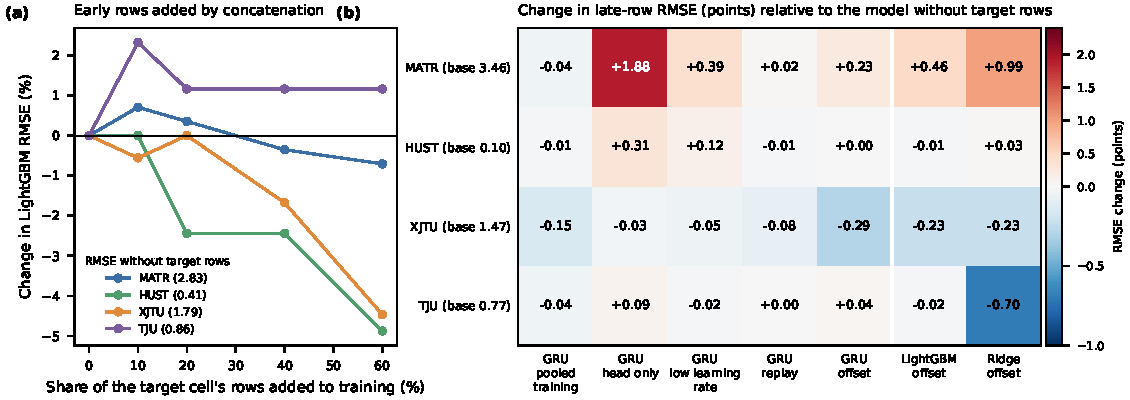
\includegraphics[width=\textwidth]{figures/fig_schedules.pdf}
\caption{Use of early rows of the target cell. (a) Change in the pooled LightGBM RMSE on the late 40\% of each fold cell when a growing share of the early rows of the cell is added to training; the legend gives the error without target rows. (b) Change in the late-row RMSE (points of SOH; blue lower, red higher) of five calibration schedules of a GRU (pooled training with the early rows added by concatenation, head only, low learning rate, replay and per-cell offset) and of the per-cell offset applied to LightGBM and ridge regression, relative to the same model trained without target rows (base error in the row labels).}
\label{fig:schedules}
\end{figure*}

No schedule improved the error consistently (Fig.~\ref{fig:schedules}). At $f=0.6$ concatenation and replay changed the GRU error by at most 0.15 points, and freezing the recurrent layers increased the error by @@ftc_matr_GRU_head_f0p6_minus_base@@ points on MATR and @@ftc_hust_GRU_head_f0p6_minus_base@@ on HUST. The sign of the effect of the offset depended on the dataset. It lowered the error of the GRU (@@ftc_xjtu_GRU_offset_f0p6_minus_base@@) and of LightGBM (@@ftc_xjtu_LightGBM_offset_f0p6_minus_base@@) on XJTU and of ridge regression on TJU, but increased the error of LightGBM (@@ftc_matr_LightGBM_offset_f0p6_minus_base@@, interval @@ftc_matr_LightGBM_offset_f0p6_minus_base_lo@@ to @@ftc_matr_LightGBM_offset_f0p6_minus_base_hi@@) and of ridge regression on MATR. On MATR the offset improved the late error of @@ob_matr_short_share@@\% of the shortest third of cells but of only @@ob_matr_long_share@@\% of the longest third, which carries @@ob_matr_long_rows@@\% of the late rows. The reason is that LightGBM underestimates the SOH of these long-lived cells early in life and overestimates it late, so that an offset from early life shifts later predictions in the wrong direction (Fig.~\ref{fig:offset}). Early labeled rows of the target cell therefore improved the best model clearly only on XJTU, where a one-parameter offset performed as well as any retraining.
\begin{figure*}[!t]
\centering
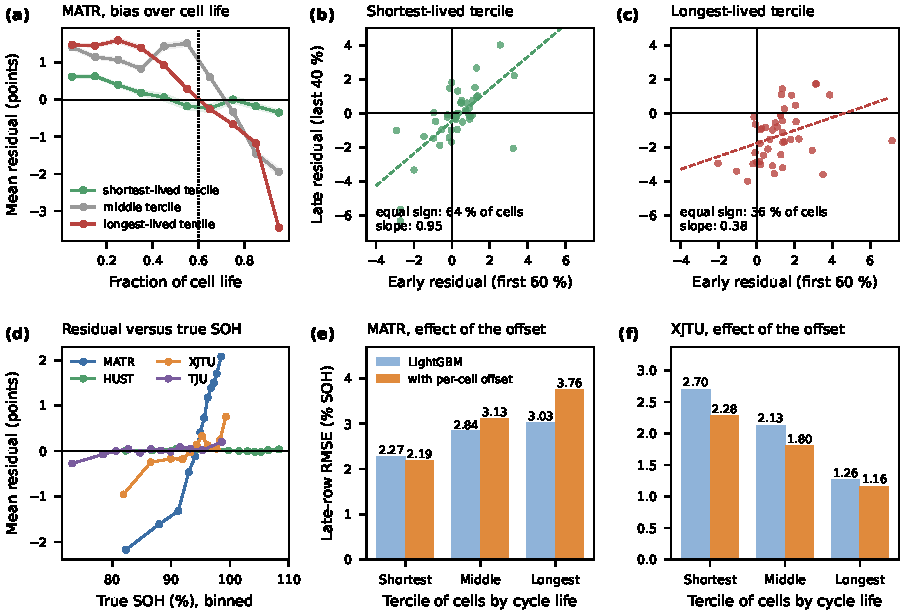
\includegraphics[width=\textwidth]{figures/fig_offset.pdf}
\caption{Mechanism of the offset results (out-of-fold predictions of LightGBM). (a) Mean residual (true minus predicted) against the fraction of cell life for the three terciles of MATR cells by cycle life; the dotted line marks the end of the early rows; bands are 95\% intervals. (b), (c) Mean late residual against mean early residual for each cell of the shortest-lived and the longest-lived third of MATR cells, with the least-squares line. (d) Mean residual against true SOH in bins, for the four larger datasets. (e), (f) Late-row RMSE of LightGBM with and without a per-cell offset (median early residual) by tercile of cycle life on MATR and XJTU.}
\label{fig:offset}
\end{figure*}

To examine whether the findings depend on the architecture, we added four further networks (Table~\ref{tab:arch}): an LSTM \cite{hochreiter1997}, a temporal convolutional network (TCN \cite{lea2017}; three causal dilated layers), a multilayer perceptron on the flattened window of ten cycles, and a GRU with a window of 30 cycles. We also added two further seeds of the GRU and the transformer.
\begin{table}[!tb]
\caption{RMSE (\% SOH) of further architectures under P0, P2, P3 and the temporal split (last 40\% of each cell). One untuned run per architecture; seed 0 for the GRU and the transformer.}
\label{tab:arch}
\centering
\fitcol{tables/arch.tex}
\end{table}

The question with the highest error depends on the architecture. On MATR and HUST the temporal error was higher than the held-out-group error for every architecture, on XJTU for all except the TCN and the window MLP, and on TJU only for the transformer. On HUST the window MLP and the TCN forecast almost as accurately as ridge regression (@@arch_hust_WinMLP_PT@@ and @@arch_hust_TCN_PT@@ against @@arch_hust_Ridge_PT@@), whereas the GRU, the LSTM and the transformer did not. The difficulty ordering from random folds to a new cell to a new group held on MATR, XJTU and TJU for all architectures.

Seed variation is comparable to many differences between models. The GRU P3 error on XJTU ranged from @@seed_xjtu_GRU_P3_min@@ to @@seed_xjtu_GRU_P3_max@@ across three seeds, so single-run rankings among networks are not reliable. The median range over three seeds was @@ss_P2_med@@, @@ss_P3_med@@ and @@ss_PT_med@@ points under P2, P3 and the temporal split. Whether the temporal error exceeded the held-out-group error was the same in all seeds in @@ss_ptp3_consistent@@ of @@ss_ptp3_cases@@ combinations. For the tuned variants (hidden size and learning rate chosen on an inner validation set; Table~\ref{tab:tunedarch}) this statement was less stable. It held in all three seeds, or in none, in @@tss_ptp3_consistent@@ of @@tss_ptp3_cases@@ combinations and in only @@tss_ptp3_xjtu@@ of @@tss_ptp3_xjtu_n@@ on XJTU, where the two errors are of similar size. Tuning did not alter the overall picture: it lowered the GRU error clearly only on HUST and increased it under P3 on MATR and XJTU. With F2 inputs a GRU had the lowest error on HUST but a higher P3 error than LightGBM on XJTU and MATR (Table~\ref{tab:f2net}). The order of models thus changed with the input as it did with the question.
\begin{table}[!tb]
\caption{RMSE (\% SOH) of tuned networks (GRU, LSTM, TCN, window MLP, CNN-GRU, GRU with attention, transformer, pooled MLP) and of the untuned CNN-GRU and GRU with attention under P2, P3 and the temporal split. Seed 0 of the tuning run.}
\label{tab:tunedarch}
\centering
\fitcol{tables/tuned_arch.tex}
\end{table}
\begin{table}[!tb]
\caption{RMSE (\% SOH) with F2 inputs for ridge regression, LightGBM and a GRU under P2, P3 and the temporal split (rows with an F2 feature vector).}
\label{tab:f2net}
\centering
\fitcol{tables/f2_networks.tex}
\end{table}

The findings for the pooled models thus carry over to the networks in three respects: the difficulty ordering, the high error of forecasting and the absence of a benefit from early rows. They do not carry over to the ranking of models, which changed with the question. Forecasting was more difficult than a held-out group for LightGBM and the transformer on all four datasets, for the GRU and the LSTM on three and for the TCN and the window MLP on two. The difficulty of a temporal split is therefore a property of a model and a dataset, not of the question alone.

\subsubsection{Stability of Model Rankings and Calibration of the Inference}
\label{sec:res_calib}
\label{sec:res_rank}
\label{sec:res_policy}
We first checked the inference of Section~\ref{sec:design}. We exchanged the two models of each pair among the four main models at random within every unit (300 draws per pair), which creates a null without any difference between them (Table~\ref{tab:nullcal}). The percentile cluster bootstrap rejected a nominal 5\% test in @@cal_cell_boot_min@@ to @@cal_cell_boot_max@@\% of the draws with 55 to 135 cells, in @@cal_P3_boot_min@@ to @@cal_P3_boot_max@@\% with six to eleven groups and in @@pw_null_g3@@\% with three groups. The sign-flip randomization test rejected in at most @@cal_perm_max@@\% in any setting.
\begin{table}[!tb]
\centering
\caption{Rejection rate (\%) of a nominal 5\% test when the two models of a pair are exchanged at random within every unit (mean over the six pairs among ridge regression, LightGBM, GRU and transformer; 300 draws per pair).}
\label{tab:nullcal}
\scriptsize
\fitcol{tables/calibration.tex}
\end{table}

The power of the randomization test depends on the number of groups (Table~\ref{tab:power}; $G$ groups drawn from the 11 TJU groups and the 70 MATR policies, four tabular models compared in pairs). No rejection is possible with fewer than six groups. On TJU the power was @@pw_tju_6@@ with six groups and @@pw_tju_8@@ with eight. On the MATR policies it stayed below 0.02 at every $G$, because the pooled differences were small compared with the heavy tail of the per-policy errors.
\begin{table*}[!t]
\centering
\caption{Power and size with $G$ groups drawn from the 11 TJU groups and the 70 MATR policies (mean over six model pairs). Rand.: share of draws with $p<0.05$ and the correct sign in the sign-flip randomization test; boot.: the same for the percentile bootstrap interval; null: rejection rate (\%) of the bootstrap when the two models are exchanged within every group. Smallest $p$: $2^{1-G}$, the lowest two-sided $p$-value that the randomization test can give.}
\label{tab:power}
\scriptsize
\fitwide{tables/power.tex}
\end{table*}

Across all datasets and regimes (Fig.~\ref{fig:ranking}), @@flips_total@@ combinations of a model pair and a pair of protocols showed a sign change of the RMSE difference, and after Holm correction @@holm_total@@ remained supported (Table~\ref{tab:holm}). They are two model pairs on HUST with tuned hyperparameters, LightGBM against random forest and random forest against ridge regression, whose order under P0 is reversed under P2 and P3 by at most 0.16 points. None of the sign changes on TJU (11 groups), XJTU or MATR (three batches or five rate bins, too few for the criterion) remained. The lower pooled error of ridge regression under leave-one-batch-out on MATR is not a supported reversal either, because boosted trees were more accurate in two of the three batches.
\begin{figure*}[!t]
\centering
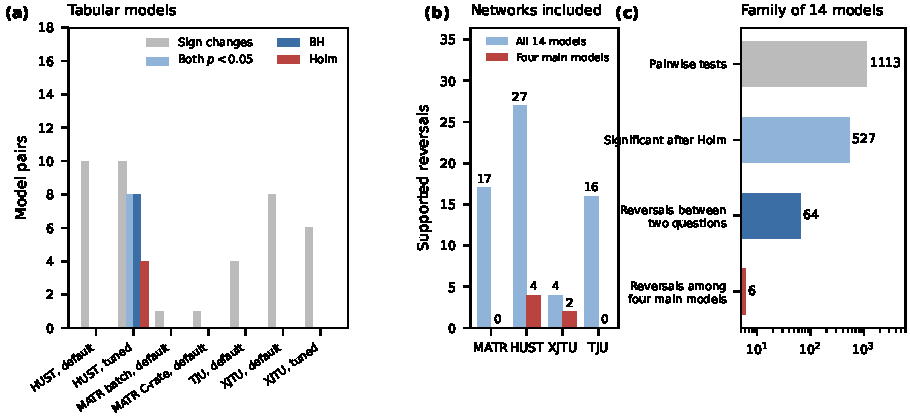
\includegraphics[width=\textwidth]{figures/fig_ranking.pdf}
\caption{Stability of model rankings. (a) For the tabular models, the number of model pairs whose RMSE difference changes sign between two protocols, the number for which both differences have $p<.05$ in the randomization test, and the number that remain after Benjamini--Hochberg (BH) and Holm correction. (b) Supported reversals between two questions in the family of 14 models, by dataset, for all models and for the four main models. (c) Filtering of the 1113 pairwise tests of the 14-model family.}
\label{fig:ranking}
\end{figure*}
\begin{table}[!tb]
\centering
\caption{Ranking changes supported after Holm correction. $\Delta_1$ and $\Delta_2$ are RMSE$_A$ $-$ RMSE$_B$ under the first and second protocol.}
\label{tab:holm}
\scriptsize
\fitcol{tables/holm.tex}
\end{table}

Adding the networks (14 models), @@g33_holm@@ of @@g33_tests@@ pairwise tests were significant after Holm correction within each dataset and question. In addition, @@g33_rev_all@@ pairs changed the sign of their difference between two questions with both questions significant. No P3 comparison in the family of 91 pairs remained significant, because with six to eleven groups the smallest attainable $p$-value does not clear 0.05/91. One family over all datasets, questions and pairs gave @@gl_holm@@ significant tests and @@gl_rev@@ sign changes.

Among the four main models (ridge regression, LightGBM, GRU, transformer), tested as the primary family of six pairs per dataset and question, @@g33_main_rev@@ changes were supported, on HUST (@@g33_main_rev_hust@@) and XJTU (@@g33_main_rev_xjtu@@). On XJTU ridge regression had a higher error than LightGBM under P0 and P2 and a lower error under the temporal split (@@tmpd_xjtu_PT@@, interval @@tmpd_xjtu_PT_lo@@ to @@tmpd_xjtu_PT_hi@@). On HUST the GRU had a lower error than ridge regression under P0 to P3 and a much higher error under the temporal split (@@g33_hust_GRU_Ridge_PT@@). Changes in model order were thus infrequent among tabular models and more frequent when the models differ in how they extrapolate. Rankings read from pooled errors or from fewer than six groups are not reliable.

To obtain a larger number of groups, we held out each of the 70 charging policies of MATR in turn (@@policy_single@@ of them a single cell). Ridge regression had the lowest pooled error (Table~\ref{tab:policy}: @@policy_ridge_p3@@ against @@policy_lgb_p3@@ for LightGBM), but the difference is not supported (@@policy_delta@@ points, $p=@@policy_p@@$). Ridge regression is more accurate than LightGBM in only @@policy_ridge_wins@@ of the 70 policies. The pooled value reflects a heavy tail: the five policies with the largest errors account for @@policy_top5_lgb@@\% of the squared error of LightGBM but @@policy_top5_ridge@@\% of that of ridge regression. Rankings by pooled error and by typical group therefore disagree, and per-group errors should be reported.
\begin{table*}[!t]
\centering
\caption{MATR, F1 features: pooled RMSE (\% SOH) for P0, P2 and leave-one-charging-policy-out (P3, 70 groups), with group-held-out inner tuning, and the distribution of the P3 error over policies.}
\label{tab:policy}
\scriptsize
\fitwide{tables/policy.tex}
\end{table*}

\subsubsection{Hyperparameter Selection and Preprocessing}
\label{sec:res_tuning}
\label{sec:res_selection}
Table~\ref{tab:tuning} compares fixed hyperparameters with two nested schemes under P3 (four inner seeds). Holding out groups in the inner folds lowered the error where the inner scheme mattered most. For XGBoost on XJTU the pooled RMSE was @@xjtu_xgb_default@@ with fixed settings, @@xjtu_xgb_cell@@ with cell-held-out and @@xjtu_xgb_grp@@ with group-held-out inner folds. For LightGBM on MATR with charge-rate bins the corresponding values were @@crate_lgb_default@@, @@crate_lgb_cell@@ and @@crate_lgb_grp@@. Tuning also benefits the protocols unequally. On MATR it lowered the LightGBM error by @@tune_matr_LightGBM_P0@@\% under P0 but only @@tune_matr_LightGBM_P3@@\% under P3. On XJTU it lowered the error by @@tune_xjtu_LightGBM_P0@@\% under P0 and increased it by @@tune_xjtu_LightGBM_P3@@\% under P3.
\begin{table*}[!t]
\centering
\caption{P3 pooled RMSE (\% SOH): fixed hyperparameters and nested selection; mean (SD) over four inner-search seeds.}
\label{tab:tuning}
\scriptsize
\fitwide{tables/tuning.tex}
\end{table*}

The second internal threat is selecting the single configuration with the lowest pooled error on the folds that are subsequently reported. We define the optimism as the relative reduction of the pooled error compared with nested selection with cell-held-out inner folds. It was negligible under random folds (median @@opt_P0_med@@\%) and under cell-disjoint folds (median @@opt_P2_med@@\%). Under held-out groups it reached @@opt_P3_max@@\% on XJTU (Table~\ref{tab:selection}) and @@sx_tju_P3_max@@\% on TJU.

Held-out-group results rest on one partition. We therefore repeated the experiment with random assignments of whole groups to outer folds (five to eight partitions per dataset; Table~\ref{tab:selpart}). Selection on the reported folds gave a lower pooled error than nested selection in @@sp_pos@@ of @@sp_n@@ combinations of partition and model, with a maximum optimism of @@sp_max@@\%. The optimism was concentrated in the tree ensembles and in the datasets whose groups are remote from one another (mean over partitions @@sp_xjtu_XGBoost_opt@@\% for XGBoost and @@sp_xjtu_LightGBM_opt@@\% for LightGBM on XJTU, and @@sp_tju_XGBoost_opt@@\% and @@sp_tju_LightGBM_opt@@\% on TJU, against at most @@sp_hust_LightGBM_opt@@\% on HUST). This is consistent with the distance of the held-out groups from the training data (Section~\ref{sec:res_typology}). The optimism also varied strongly between partitions of one dataset, so a single partition can understate or overstate it.
\begin{table*}[!t]
\centering
\caption{P3-type evaluation with repeated random assignments of whole groups to outer folds: pooled RMSE (\% SOH; mean and standard deviation over partitions) with fixed hyperparameters, nested selection (group-held-out inner folds) and selection on the reported folds. Optimism is the relative reduction from the nested to the reported-fold selection, with its range over partitions; the last column counts partitions with a positive optimism.}
\label{tab:selpart}
\scriptsize
\fitwide{tables/selection_partitions.tex}
\end{table*}

Preprocessing fitted before splitting was not material for these models and features. Fitting the imputer and standardizer of ridge regression on all rows changed the pooled RMSE by at most @@prep_max_abs@@ points (@@prep_max_where@@) and by at most @@prep_second@@ points elsewhere. For the GRU on XJTU and TJU the change was @@pp_min@@ to @@pp_max@@ points under P2 and P3, which is comparable to the seed-to-seed spread of Section~\ref{sec:res_arch}. The inner-fold scheme and selection on the reported folds are evaluation choices that should be reported.
\begin{table*}[!t]
\centering
\caption{P3 pooled RMSE (\% SOH): fixed hyperparameters, nested selection and selection on the reported folds. Optimism is the relative reduction from nested selection with cell-held-out inner folds to selection on the reported folds.}
\label{tab:selection}
\scriptsize
\fitwide{tables/selection.tex}
\end{table*}

\subsection{Construct Validity}
\label{sec:construct}
Construct validity concerns the quantities from which the error is computed: the capacity reference that defines the label, and the input features, some of which can encode the label.

\subsubsection{Label Reference and Capacity-Derived Inputs}
\label{sec:res_label}
Capacity-based SOH is the ratio of a measured capacity to a reference capacity. A widely used benchmark platform predicts the ratio of the observed discharge capacity to the nominal capacity because reference performance tests are not always available in public datasets \cite{zhang2024}. The choice of nominal capacity therefore affects both the label and the error in percentage points.

Adding the charge capacity of the cycle (F3) lowered the LightGBM error under random folds on MATR from @@matr_lgb_f1_p0@@ to @@matr_lgb_f3_p0@@ (Table~\ref{tab:coupling}). On HUST the difference between the charge and the discharge capacity of the same cycle has a standard deviation of only @@hust_qchg_sd_mAh@@\,mAh, so the label is almost contained in the input. The definition of the label also changes the error (Table~\ref{tab:labels}). The reference label increased the LightGBM error on TJU from @@lab_tju_LightGBM_rated_P0@@ to @@lab_tju_LightGBM_ref_P0@@ under P0 and on HUST from @@hust_lgb_rated_p0@@ to @@hust_lgb_ref_p0@@. Dividing by a different nominal capacity rescales the error in percentage points by the ratio of the two capacities. Errors from different studies are therefore comparable only if the reference capacity is stated.
\begin{table}[!tb]
\centering
\caption{RMSE (\% SOH) with F1 (left) and F3 = F1 + charge capacity (right); P3a is leave-one-group-out.}
\label{tab:coupling}
\scriptsize
\fitcol{tables/coupling.tex}
\end{table}
\begin{table}[!tb]
\centering
\caption{RMSE (\% SOH) under the rated label (left) and the reference label (right), fixed hyperparameters, F1.}
\label{tab:labels}
\scriptsize
\fitcol{tables/labels.tex}
\end{table}

The effect of a capacity-derived input is not general. On XJTU the charge capacity tracks the label closely in batches 1 to 5 but not in batch 6 (correlation @@qb_corr_6@@). Adding it (Table~\ref{tab:f3xjtu}) lowered the LightGBM error under random folds from @@f3x_LightGBM_F1_P0@@ to @@f3x_LightGBM_F3_P0@@ but increased it under held-out batches from @@f3x_LightGBM_F1_P3@@ to @@f3x_LightGBM_F3_P3@@. On TJU, where the charge capacity correlates @@f3t_corr@@ with the label, it lowered the LightGBM error under both P0 and P3 (under P3 from @@f3t_LightGBM_F1_P3@@ to @@f3t_LightGBM_F3_P3@@). An input that encodes the label in the training groups can thus mislead in a held-out group where the relation does not hold. In batch 6 the charge capacity falls short of the label (on average @@bv_def6@@\,Ah, against at most @@bv_def13@@\,Ah in batches 1 to 3). The cells enter the charge only partly discharged (Spearman correlation @@bv_rho6@@ with the voltage at the start of the charge). We did not identify the cause of the incomplete discharge.
\begin{table}[!tb]
\centering
\caption{XJTU and TJU: pooled RMSE (\% SOH) with F1 (left) and with F3 = F1 plus charge capacity (right).}
\label{tab:f3xjtu}
\scriptsize
\fitcol{tables/f3xjtu.tex}
\end{table}

A small error therefore cannot be interpreted without the reference capacity and the list of inputs.

\subsection{External Validity}
\label{sec:external}
External validity concerns whether the error carries over to other cells, conditions and settings. We examine the meaning and distance of held-out groups and the dependence of conclusions on the feature set. With the present data we cannot measure the difference between laboratory and field conditions.

\subsubsection{Held-Out Groups and Distance from the Training Data}
\label{sec:res_typology}
\label{sec:res_support}
Q4 is operationalized by P3, but the held-out groups differ in kind between the datasets (Table~\ref{tab:typology}). A MATR batch is largely an unseen set of charging policies, and a charge-rate bin or a policy is a charging protocol. The HUST identifier groups share one charging protocol. An XJTU batch is a charge and discharge strategy, and a TJU group combines a cell type with a cycling condition. For each grouping, we related the ratio of the LightGBM or ridge error under leave-one-group-out to that under P2 on the same rows to the distance ratio. The distance ratio is the median distance of the held-out rows to the nearest training row in the standardized F1 space, divided by the same median under P2. A value of one means that the held-out rows are no more remote than those of a new cell. We added alternative groupings. For TJU they are the held-out cell type, cycling temperature and charging rate. For all four datasets we also held out a cluster of cells in input space (k-means, five clusters, on the median standardized F1 values over cycles 2 to 30 of each cell).
\begin{table*}[!t]
\centering
\caption{Held-out groups in the four datasets and in alternative groupings. Groups: number of held-out groups; distance ratio: median distance of the held-out rows to the nearest training row in the standardized F1 space relative to P2; P3/P2: pooled RMSE under leave-one-group-out relative to P2 on the same rows. Default hyperparameters, F1 features, rated label.}
\label{tab:typology}
\scriptsize
\fitwide{tables/typology.tex}
\end{table*}
\begin{figure*}[!t]
\centering
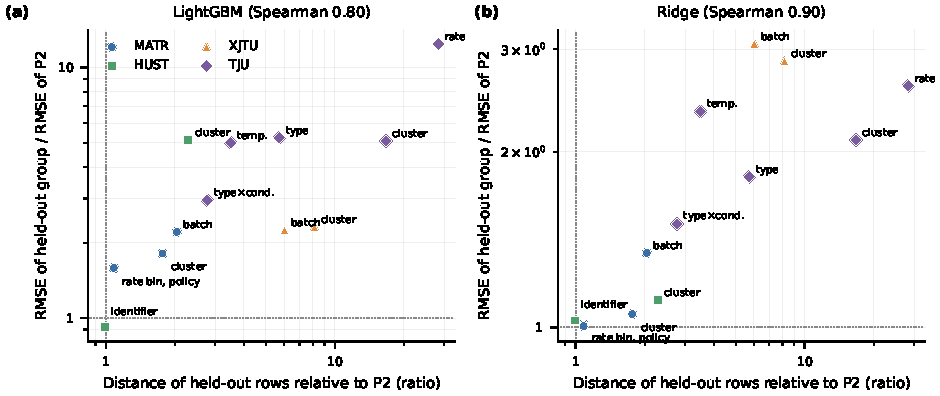
\includegraphics[width=\textwidth]{figures/fig_typology.pdf}
\caption{Error penalty of a held-out group against its remoteness. Each point is one grouping (Table~\ref{tab:typology}); the abscissa is the median distance of the held-out rows to the nearest training row relative to the same distance under P2, and the ordinate the RMSE under leave-one-group-out relative to that under P2 on the same rows. (a) LightGBM. (b) Ridge regression. The Spearman correlation over the @@gt_n@@ groupings is given in the panel titles.}
\label{fig:typology}
\end{figure*}

Across the @@gt_n@@ groupings, the ratio of the LightGBM error to its P2 error ranged from @@gt_hust_identifier_group_ratio@@ for the HUST identifier groups to @@gt_tju_charging_rate_ratio@@ for the held-out charging rate of TJU, and the distance ratio from @@gt_hust_identifier_group_dist@@ to @@gt_tju_charging_rate_dist@@ (Fig.~\ref{fig:typology}). The rank correlations were @@gt_rho_lgb@@ for LightGBM and @@gt_rho_ridge@@ for ridge regression. The HUST identifier groups are as close to the training data as a new cell, which confirms that HUST P3 is a cell-disjoint design. One dataset can also pose very different Q4 questions. On MATR the error ratio was @@gt_matr_charging_policy_ratio@@ for held-out policies and @@gt_matr_batch_ratio@@ for batches, and on TJU @@gt_tju_type_x_condition_ratio@@ for type by condition and @@gt_tju_charging_rate_ratio@@ for charging rate. Remoteness does not explain everything: the XJTU batches had a distance ratio of @@gt_xjtu_batch_dist@@ but an error ratio of only @@gt_xjtu_batch_ratio@@. The penalty therefore also depends on how the model responds to the shift.

At the level of rows, we gave each evaluation row the ratio of its mean distance to the ten nearest training rows to the median of the same quantity over reference training rows. This follows the spirit of the ``area of applicability'' of a model \cite{meyer2021}. We binned rows by terciles of this ratio (Fig.~\ref{fig:distance}, Table~\ref{tab:support}). Under P3 on MATR and HUST the difference between ridge regression and LightGBM changes in the same direction with distance. However, the pattern differs between datasets, and with a Mahalanobis distance MATR under P3 differed from the pattern above. Feature distance therefore provides only a partial account.
\begin{figure*}[!t]
\centering
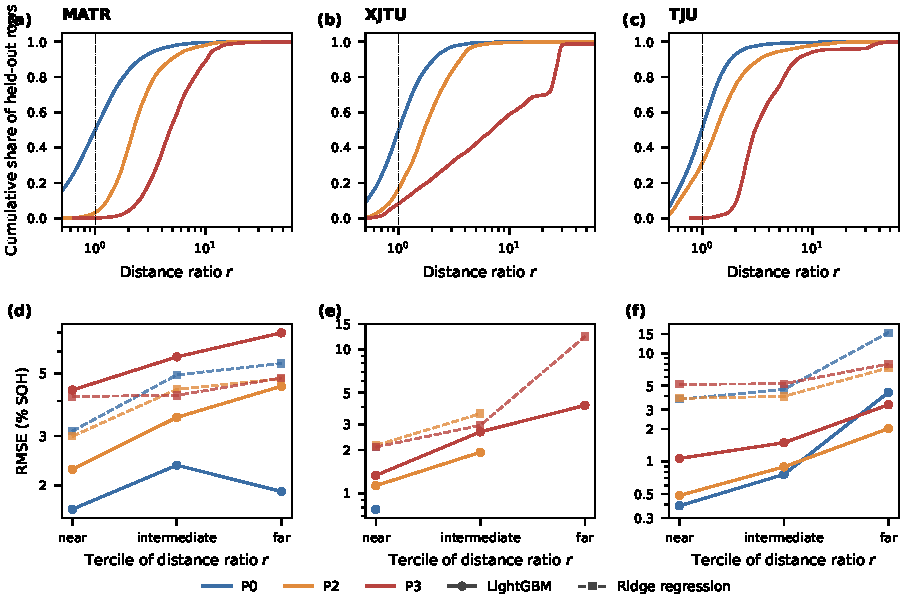
\includegraphics[width=\textwidth]{figures/fig_distance.pdf}
\caption{Distance of the evaluation rows from the training rows. (a)--(c) Empirical distribution of the distance ratio $r$ (mean distance to the ten nearest training rows divided by the median of the same quantity for reference training rows; features only) of the held-out rows under P0, P2 and P3. (d)--(f) Pooled RMSE of LightGBM (solid) and ridge regression (dashed) in terciles of $r$ for each protocol; the thresholds are fixed from the P3 rows.}
\label{fig:distance}
\end{figure*}
\begin{table*}[!t]
\centering
\caption{RMSE$_\mathrm{Ridge}-$RMSE$_\mathrm{LightGBM}$ (points of SOH) by distance bin, with 95\% cluster-bootstrap intervals; negative values favor ridge regression.}
\label{tab:support}
\scriptsize
\fitwide{tables/support.tex}
\end{table*}

\subsubsection{Feature Set and Field Conditions}
\label{sec:res_curve}
\label{sec:res_field}
Replacing F1 by F2 (Table~\ref{tab:curve}) alters some conclusions. On MATR, LightGBM was more accurate than ridge regression under all three protocols (P3: @@curve_matr_LightGBM_P3@@ against @@curve_matr_Ridge_P3@@), whereas with F1 the pooled P3 error of ridge regression was lower. In contrast, on HUST the F2 features were less informative, and the order of random forest and ridge regression changed between P0 and P3, the only supported ranking change with F2 (Holm, @@curve_holm@@ pair). With tuned hyperparameters the MATR conclusion was unchanged, but on HUST tuning reversed the order of LightGBM and ridge regression (P3 @@f2t_hust_LightGBM_P3_tuned@@ against @@f2t_hust_Ridge_P3_tuned@@, against @@f2t_hust_LightGBM_P3_default@@ and @@f2t_hust_Ridge_P3_default@@ with default settings). A comparison of models does not necessarily transfer from one feature set to another.
\begin{table}[!tb]
\centering
\caption{Pooled RMSE (\% SOH) with charge-curve features F2, fixed hyperparameters.}
\label{tab:curve}
\scriptsize
\fitcol{tables/curve.tex}
\end{table}

Field data are outside the present data. Pozzato \textit{et al.} concluded from one year of field data from an electric-vehicle pack that laboratory data collected at constant temperature are a weak basis for robust SOH estimators \cite{pozzato2023}. A comparison of six evidence sources reported that ``battery performance metrics are conditional on the duty pattern that generated them'' \cite{zhao2026}. All five datasets used here are laboratory data. A claim about transfer beyond them therefore requires evidence from the target setting, such as field data with independent reference capacities.

\section{Implications for Model Families}
\label{sec:families}
Many recent studies present a new architecture as their contribution \cite{aud24,aud26,aud25}. An improvement over baselines can be interpreted only if the baselines were evaluated on the same held-out unit, with the same tuning effort and the same label. This section relates the designs in Table~\ref{tab:practice} to our measurements. It makes no statement about the accuracy of any cited model.

Transformer and state-space models are evaluated on small sets of cells \cite{aud24,aud26}. The number of independent training units then equals the number of cells, irrespective of the number of cycles. In our experiments the rank of a GRU and a small transformer relative to LightGBM and ridge regression changed with the question, and the high error of forecasting depended on the architecture (Section~\ref{sec:res_neural}). The architectures we used are generic, however.

Transfer settings often fine-tune the model on a share of the target cell \cite{aud25,aud49}, train on one cell and test on others at other conditions \cite{aud31}, or train on many cells and test on others \cite{aud53}. In our experiments, adding early rows of the target cell changed the error of pooled models very little, and four fine-tuning schedules and a per-cell offset did not improve the GRU consistently (Sections~\ref{sec:res_calibration} and \ref{sec:res_schedules}). A fine-tuning claim should therefore be accompanied by a baseline that receives the same share of target-cell data. A physics-informed network such as that of \cite{wang2024} takes extracted features as input, so whether the physical structure helps depends on the feature set against which it is compared (Section~\ref{sec:res_curve}). Augmentation and simulation increase the number of training cycles \cite{aud21,aud29} but not the number of training cells. The test cells must also be kept out of the generator, as well as the predictor.

\section{Input Signals and Associated Threats}
\label{sec:signals}
The studies of Table~\ref{tab:practice} can be grouped by input signal, because the threats discussed above affect each signal differently. Features from the charge voltage curve or from incremental capacity \cite{aud17,aud12} are exposed mainly through construct validity. The way features are derived determines whether the input encodes capacity, and the model ranking depended on the feature set (Section~\ref{sec:res_curve}). Estimation from a short segment of constant-current charging \cite{aud31,aud54} or from partial charging data \cite{aud53} adds a source of shift between training and test cells. One study attributes the ``outstanding performance'' of earlier methods to ``the same cycling condition between the trained and test cells'' \cite{aud31}. The cycling condition should therefore be held out as well as the cell. Impedance-based studies use few cells \cite{aud42,aud46,aud52}, so the choice of training and test cells has a large influence. One of them tests on new cells at temperatures that also occur in training \cite{aud52}. Pack measurements \cite{aud37,aud57} and field data \cite{pozzato2023,zhao2026} differ in the origin of the label: when no reference capacity test is available, the label is an estimate. These statements rest on the designs and on our experiments with charge-curve features. We did not measure the other signals.

\section{Scope of the Evidence}
\label{sec:discussion}
Our measurements support the following findings, each of which concerns the correspondence between the question and the reported error. First, the error of a flexible model depends strongly on the question, whereas that of ridge regression depends much less. A small gap between questions is therefore not a sign of a safe design (Section~\ref{sec:res_protocol}). Second, a temporal split poses a different and, for LightGBM on all datasets, more difficult question than a held-out cell. The difficulty is accounted for by the absence of late-life data from the other cells in the training pool, not by the temporal order or the missing history of the target cell. Avoiding temporal leakage therefore does not make a temporal split a safe design. Third, early rows of the target cell contributed little or nothing in most settings, whatever the schedule, whereas late-life rows of other cells did contribute.

Fourth, after accounting for the number of independent groups and for multiple comparisons with tests that keep their size, supported changes in the order of two tabular models between protocols were few (@@holm_total@@ of @@flips_total@@) and confined to small differences on HUST with tuned hyperparameters. Among ridge regression, LightGBM, a GRU and a transformer, @@g33_main_rev@@ changes between questions were supported, on HUST and XJTU. In addition, the reported error depended on whether errors are pooled over cycles or averaged over cells (which reordered @@mac_pct@@\% of model pairs) and on what the held-out group represents (an error ratio to a new cell from @@gt_hust_identifier_group_ratio@@ to @@gt_tju_charging_rate_ratio@@ for LightGBM). The hyperparameter selection, the reference of the label and the presence of an input that encodes capacity each changed the error, in some cases by more than the difference between models.

These findings are consistent with the position of \cite{sohail2026} and \cite{rizanov2026} that errors depend on the protocol. They are also consistent with the indication of four NASA cells that random folds mostly measure interpolation \cite{barua2026,le2026}, and with the direction reported for random against group-wise folds \cite{maher2025} and for capacity-equivalent inputs \cite{erdogan2026}. The additional observation is that the usual expectation, in which error increases with decreasing target information and temporal splits are the safe choice, holds only in part.

We do not claim that random cycle-level splits are common in the literature. The passages we read for Table~\ref{tab:practice} often do not settle whether cycles of one cell reach both the training and the test set, and the only prevalence estimate we know of comes from a concurrent, unreviewed survey \cite{erdogan2026}. P0 is a reference condition, which we use because \cite{sohail2026} rank random splits as the lowest-rigor protocol. We also do not claim that held-out evaluation measures field performance. All five datasets are laboratory data, and the cited field studies \cite{pozzato2023,zhao2026} point to differences that our design cannot examine.

\section{Reporting Recommendations}
\label{sec:recs}
A reporting checklist is useful only if each item can be traced to an effect that its omission would hide. The lists of \cite{sohail2026} and \cite{rizanov2026} already ask for the dataset, the target definition, the order of preprocessing and the split. Table~\ref{tab:checklist} adds the items for which our reading of the studies (Section~\ref{sec:practice}) and our experiments (Section~\ref{sec:analysis}) indicate that omission changes the interpretation of a reported error. For each item it gives the measured effect and the section in which the item is examined. None requires more data than a study already has.

\begin{table*}[!t]
\caption{Reporting checklist for studies of data-driven SOH estimation. The last column gives the section in which the item is examined.}
\label{tab:checklist}
\centering
\footnotesize
\begin{tabular}{p{0.03\textwidth}p{0.30\textwidth}p{0.45\textwidth}p{0.10\textwidth}}
\toprule
 & Report & Why (what changes if it is missing) & Section \\
\midrule
1 & The task: estimation for a cell never seen, forecasting of later cycles of a cell, or calibration with data of the target cell & The tasks answer different questions. The error under random folds, which include cycles of the evaluated cell in training, differed from that under held-out batches by up to a factor of @@matr_LightGBM_ratio_P3_P0@@, and a temporal split gave a still larger error for tree ensembles. Early data of the target cell added little to a pooled model, and the greater error of a forecast was accounted for by the missing late-life data of other cells, which a report should state. A study that mixes the tasks cannot be compared with others & \ref{sec:practice}, \ref{sec:res_protocol}, \ref{sec:res_temporal}, \ref{sec:res_factorial} \\
2 & The independent unit that is held out (cycle, cell, batch, condition, dataset) and the number of such units & The pooled error describes only the held-out units, a ranking cannot be tested with fewer than six groups (about eight when several models are compared), and whether the error is pooled over cycles or averaged over cells reordered @@mac_pct@@\% of model pairs & \ref{sec:res_protocol}, \ref{sec:res_macro}, \ref{sec:res_calib}, \ref{sec:res_rank} \\
3 & Uncertainty computed over that unit, and a correction for the number of model comparisons & Cell-level intervals ignore the correlation within a group, a percentile cluster bootstrap rejected a true null in @@cal_P3_boot_min@@ to @@cal_P3_boot_max@@\% of draws with six to eleven groups (an exact randomization test kept its size), and unadjusted comparisons produce many apparent changes in ranking & \ref{sec:res_calib}, \ref{sec:res_rank}, \ref{sec:res_policy} \\
4 & The hyperparameter-selection scheme, the unit held out in the inner folds, and whether the reported folds were used for selection & Selection on the reported folds lowered the apparent error by up to @@opt_P3_max@@\% in one case, and inner folds that hold out cycles do not mimic deployment & \ref{sec:res_tuning}, \ref{sec:res_selection} \\
5 & The reference capacity, its source, and the error in capacity units when the reference differs from the rated value & The error in percentage points depends on the reference; a per-cell reference changed the error several-fold on HUST & \ref{sec:res_label} \\
6 & Whether any input is derived from capacity, and results without such inputs & A capacity-derived input removed most of the error on two datasets and increased the held-out-batch error on a third & \ref{sec:res_label} \\
7 & A simple baseline (for example ridge regression) with the same tuning effort and, for fine-tuned models, the same share of target-cell data & On the largest dataset, the linear baseline was not less accurate than boosting once all 70 policies were held out & \ref{sec:res_policy}, \ref{sec:families} \\
8 & Results for more than one feature set when a conclusion about model families is drawn & The order of ridge regression and LightGBM depended on the feature set & \ref{sec:res_curve} \\
9 & Preprocessing fitted on training data only, with seeds, code and the exact partition & Fitting simple preprocessing on all rows had no material effect for the models examined, but the order of preprocessing and the partition itself are sometimes not recoverable from the text & \ref{sec:res_selection}, \ref{sec:practice} \\
10 & The range of operating conditions, the type of shift that a held-out group represents and the distance of the test data from the training data & The error ratio to a new cell ranged from @@gt_hust_identifier_group_ratio@@ to @@gt_tju_charging_rate_ratio@@ across groupings, and feature distance accounted for part of this penalty but not for all of it & \ref{sec:res_typology}, \ref{sec:res_support} \\
11 & For neural models, several seeds and more than one architecture, and the calibration schedule with a per-cell offset baseline & The range of the P3 error over three seeds had a median of @@ss_P3_med@@ points for untuned and @@tss_P3_med@@ for tuned networks but reached @@ss_P3_max@@ and @@tss_P3_max@@ points in single cases, which is comparable to or larger than the differences between neighboring architectures, and the effect of fine-tuning changed sign between datasets & \ref{sec:res_schedules}, \ref{sec:res_arch} \\
\bottomrule
\end{tabular}
\end{table*}

The items do not carry equal weight in our data. The question and the held-out unit (items 1 and 2) changed the error by up to a factor of @@matr_LightGBM_ratio_P3_P0@@. A capacity-derived input (item 6) removed most of the error on two datasets. The reference capacity (item 5) changed the error several-fold on HUST, and selection on the reported folds (item 4) lowered the apparent error by up to @@opt_P3_max@@\%. In contrast, fitting simple preprocessing on all rows (item 9) had no material effect. A study with limited space can therefore give priority to items 1, 2, 4, 5 and 6. The checklist is derived from five public laboratory datasets and from the designs in Table~\ref{tab:practice}. It describes what we found to matter there and contains no items for field data. Applying it does not make a design appropriate, but it makes explicit the question that the design answers.

\section{Limitations}
\label{sec:limits}
Our data are four public laboratory datasets with at most 135 cells and a four-cell reference. The natural groupings for P3 contain three to eleven groups, which limits tests of rankings (Section~\ref{sec:res_calib}), and the alternative groupings of Section~\ref{sec:res_typology} have three to five groups each. XJTU labels exist only for cycles with measured capacity, and the rated label of TJU is a cell-type reference, not a datasheet value. Features are cycle-level summaries or charge-curve checkpoints, and the hyperparameter grids are small. We ran the networks at a single training share (60\%) and the charge-curve experiments once.

Three explanations remain incomplete. We do not know how missing late-life coverage raises the error on rows within the training range (MATR, TJU), what causes the residual temporal error on TJU, or why a per-cell offset increases the error of the long-lived MATR cells.

The sign-flip test assumes that two models are exchangeable within every unit under the null hypothesis, which is stronger than equal expected error. Our statements about model families are arguments based on the present designs and experiments. They are not tests of the cited models.

The limitations affect the strength of the statements more than their direction. Field data with independent reference capacities, more datasets with distinct conditions and more held-out groups, and waveform-based inputs evaluated under the same protocol comparison would reduce them most.

\section{Conclusion}
\label{sec:conclusion}
A reported SOH error answers a question that is defined by what the model has seen of the target and by what it is asked to predict. We distinguished five such questions, mapped 40 recent studies onto them, and measured all five on the same rows of four public datasets with 55 to 135 cells and a four-cell reference dataset. Small or concurrent studies had already indicated that cell-held-out testing increases the error and that capacity-equivalent inputs inflate accuracy \cite{le2026,barua2026,maher2025,erdogan2026}. Our contribution lies in the comparison across questions, with inference at the level of the cell or group by tests that keep their size.

The main results are as follows. Forecasting the later life of a cell can be more difficult than estimating a new cell. This difference is accounted for by the missing late-life data of other cells, not by the temporal order or the absence of the target cell, and early rows of the target cell improved the error clearly on one dataset only. Among tabular models most changes in model order between protocols did not remain after correction, whereas models that differ in kind showed supported changes between questions. Hyperparameter selection, label reference and capacity-derived inputs each changed the error.

The appropriate evaluation depends on the intended use. An estimator applied to cells of types and conditions present in the training data can be evaluated with held-out cells (Q3). One intended for new cell types or operating conditions should be evaluated with held-out groups (Q4), with the type of shift and the number of groups stated, since rankings based on fewer than six groups cannot be tested. One intended to forecast the aging of cells in service should be evaluated with a temporal split (Q5). In our data the main threat to such a forecast was the missing coverage of late life in the training pool, not leakage. When early data of the target cell are used (Q2), the result should be compared with a per-cell offset baseline. In all cases, a report should state the question, the held-out unit and its count, whether errors are pooled over cycles or averaged over cells, the reference capacity, the origin of the inputs and the tuning scheme. Field data with independent reference capacities remain necessary to determine how far these laboratory results transfer.

\section*{Data and Code Availability}
All five datasets are public: the NASA Prognostics Center of Excellence battery data set \cite{saha2007}; the MATR data of \cite{severson2019} (\url{https://data.matr.io/1/}); the HUST data of \cite{ma2022} (Mendeley Data, doi:10.17632/nsc7hnsg4s); the XJTU data of \cite{wang2024} (Zenodo, record 10963339); and the TJU data of \cite{zhu2022} (Zenodo, record 6405084). The scripts, fixed random seeds, extracted per-cycle features and result tables used to generate every table and figure are available at \url{https://github.com/HuyHoangLe0201/soh-validity-repro}, and the stored predictions are distributed as a release archive of that repository. Software versions: Python 3.13, scikit-learn 1.9.1, LightGBM 4.7.0, XGBoost 3.4.1, PyTorch 2.15.0.

\bibliographystyle{IEEEtran}
\bibliography{references}

\begin{IEEEbiographynophoto}{[First Author]}
[Biography to be supplied.]
\end{IEEEbiographynophoto}

\EOD
\end{document}
